\documentclass{UVKABoA4}

\usepackage{graphicx} % Standardpaket zur Grafikeinbindung
\usepackage{amsmath,amssymb} % Erweiterung des Mathematik-Modus
\usepackage[colorinlistoftodos, german]{todonotes} % Option 'disable' entfernt alle ToDos
\usepackage[absolute,overlay]{textpos}
\usepackage{vmargin}          % Adjust margins in a simple way
\usepackage{tikz}

% Toggle the following two lines to switch between english and german layout
\usepackage[english]{babel} % Neue deutsche Rechtschreibung und Silbentrennung.


\usepackage[raiselinks=true,
            bookmarks=true,
            bookmarksopenlevel=1,
            bookmarksopen=true,
            bookmarksnumbered=true,
            hyperindex=true,
            plainpages=false,
            pdfpagelabels=true,
            pdfborder={0 0 0.5}]{hyperref}


\makeatletter
\def\tagform@#1{\maketag@@@{\ignorespaces [#1]\unskip\@@italiccorr}}	% Anpassung der Formelnummerierung
\makeatother

\makeindex

\newcommand{\myname}{Forename~Surname}
\newcommand{\headtitle}{Title of thesis\\ 
                        Second title line}
\newcommand{\floatingtitle}{Title of thesis - Second title line}
\newcommand{\thesistype}{Master thesis}

\newcommand{\reviewerone}{Prof.~Dr.--Ing.~J.~M.~Zöllner}
\newcommand{\reviewertwo}{Prof.~Dr.--Ing.~R.~Dillmann}
\newcommand{\advisor}{Dipl.--Inform.~Max~Mustermann}

\newcommand{\timestart}{XX. Monat 20XX}
\newcommand{\releaseyear}{2016}
\newcommand{\timeend}{XX. Monat \releaseyear}
\newcommand{\releasemonth}{in Monat \releaseyear}


% Names of the organizations
\newcommand{\department}{\iflanguage{english}{Department of Computer Science}
                                             {Fakultät für Informatik}}
\newcommand{\institute}{\iflanguage{english}{Institute for Anthropomatics}
                                            {Institut für Anthropomatik}}
\newcommand{\fzidepartment}{Abteilung Technisch Kognitive Assistenzsysteme}
\newcommand{\fziname}{\iflanguage{english}{FZI Research Center for Information Technology}
                                          {FZI Forschungszentrum Informatik}}

% A graphic best describing your thesis
\newcommand{\titlefig}{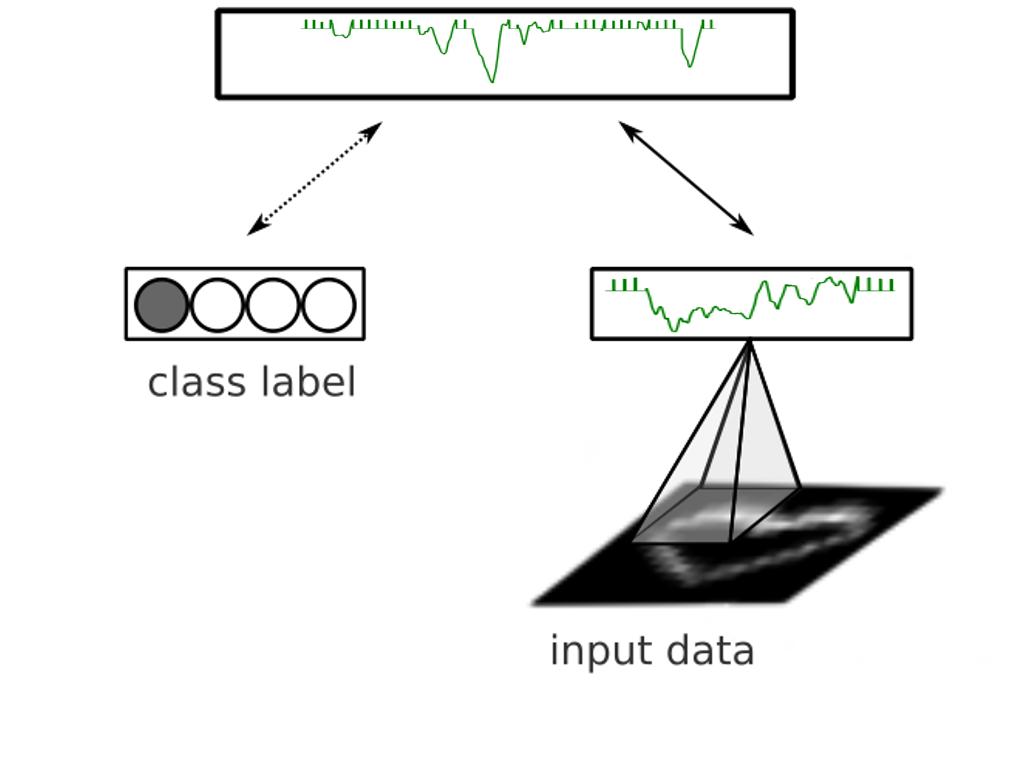
\includegraphics[width=1.0\textwidth]{graphics/not-the-final-title}}

\begin{document}

\pagenumbering{roman}
%% titlepage.tex
%%

% coordinates for the bg shape on the titlepage
\newcommand{\diameter}{20}
\newcommand{\xone}{-25}
\newcommand{\xtwo}{150}
\newcommand{\yone}{25}
\newcommand{\ytwo}{-243}

\begin{titlepage}
% bg shape
\begin{tikzpicture}[overlay]
\draw[color=gray]  
 		 (\xone mm, \yone mm)
  -- (\xtwo mm, \yone mm)
 arc (90:0:\diameter pt) 
  -- (\xtwo mm + \diameter pt , \ytwo mm) 
	-- (\xone mm + \diameter pt , \ytwo mm)
 arc (270:180:\diameter pt)
	-- (\xone mm, \yone mm);
\end{tikzpicture}
  \begin{textblock}{10}[0,0](3.35,2.55)
	  \iflanguage{english}  {
\includegraphics[width=.3\textwidth]{graphics/kitlogo_en_rgb}}
                          {
\includegraphics[width=.3\textwidth]{graphics/kitlogo_de_rgb}}
  \end{textblock}
	\changefont{phv}{m}{n}	% helvetica	
	\vspace*{2.5cm}
	\begin{center}
		\Huge{\headtitle}
		\vspace*{2cm}\\
		\Large{
			\iflanguage{english}{Master Thesis of}			
												  {Masterarbeit\\von}
		}\\
		\vspace*{1cm}
		\huge{\myname}\\
		\vspace*{1cm}
		\Large{
			\department\\ \institute\\ \iflanguage{english}{and}{und}\\ \fziname
		}
	\end{center}
	\vspace*{1.5cm}
\Large{
\begin{center}
\begin{tabular}[ht]{l c l}
  \iflanguage{english}{Reviewer}{Erstgutachter}: & \hfill  & \reviewerone\\
  \iflanguage{english}{Second reviewer}{Zweitgutachter}: & \hfill  & \reviewertwo\\
  \iflanguage{english}{Advisor}{Betreuender Mitarbeiter}: & \hfill  & \advisor\\
  % \iflanguage{english}{Second advisor}{Zweiter betreuender Mitarbeiter}: & \hfill  & \advisortwo\\
\end{tabular}
\end{center}
}


\vspace{2cm}
\begin{center}
\large{\iflanguage{english}{Research Period}{Bearbeitungszeit}: \timestart \hspace*{0.25cm} -- \hspace*{0.25cm} \timeend}
\end{center}


\begin{textblock}{10}[0,0](4,16.8)
\tiny{ 
	\iflanguage{english}
		{KIT -- University of the State of Baden-Wuerttemberg and National Research Center of the Helmholtz Association}
		{KIT -- Universität des Landes Baden-Württemberg und nationales Forschungszentrum in der Helmholtz-Gemeinschaft}
}
\end{textblock}

\begin{textblock}{10}[0,0](14,16.75)
\large{
	\textbf{www.kit.edu} 
}
\end{textblock}

\end{titlepage}

\pagestyle{empty}
\begingroup
\changefont{phv}{m}{n}
\renewcommand{\baselinestretch}{1}

\begin{titlepage}
  \parindent 0em 
  \LARGE\textbf{\floatingtitle}
  \vspace{24pt}\\
  \iflanguage{english}{by}{von}\\
  \myname \\[1.5cm]
  \begin{center}
  \titlefig\\[1cm]
  \end{center}
  \vfill
  \begin{minipage}{0.4\textwidth}
    \begin{flushleft} \large
      \LARGE\textbf{\thesistype}\\
      \LARGE\releasemonth
    \end{flushleft}
  \end{minipage}
  \begin{minipage}{0.6\textwidth}
    \begin{flushright}
      
\includegraphics[width=1.5cm]{graphics/FZI-Logo}
    \end{flushright}
  \end{minipage}
  \newpage
  \small \thesistype, FZI\\
  \department, \releaseyear\\
  Gutachter: \reviewerone, \reviewertwo
  \vfill
  \fzidepartment\\
  \fziname
  \newpage
\end{titlepage}

\endgroup

% \thispagestyle{empty}

\begin{center}
  \vspace*{\stretch{1}}
  \bfseries
  \LARGE
  \headtitle\\[0.45cm]
  \vfill
  \mdseries
  \huge
  \thesistype\\[0.8cm]
  \large
  Abteilung Technisch Kognitive Assistenzsysteme\\[0.1cm]
  Forschungszentrum Informatik\\[0.1cm]
  an der\\[0.1cm]
  Universität Karlsruhe (TH)\\
  \vfill
  von\\[0.3cm]
  \LARGE
  \myname\\
  \vfill
  \normalsize
  \begin{tabular}{p{3.5cm} p{0.4cm} p{5.5cm}}
    \textbf{Tag der Ausgabe} & : &  \timestart\\
    \textbf{Tag der Abgabe}  & : &  \closingdate\\
    & & \\
    & & \\
    & & \\
    \textbf{Betreuer} & : & \advisor \\
    \textbf{Referent} & : & Prof.~Dr.--Ing.~J.~M.~Zöllner \\
    \textbf{Koreferent} & : & Prof.~Dr.--Ing.~R.~Dillmann
  \end{tabular}
\end{center}

\parindent 1em
\affirmation

Ich versichere wahrheitsgemäß, die Arbeit selbstständig angefertigt, alle benutzten Hilfsmittel vollständig und genau angegeben und alles kenntlich gemacht zu haben, was aus Arbeiten anderer unverändert oder mit Abänderungen entnommen wurde.

\vspace{2cm}
\begin{flushright}\noindent
    Karlsruhe,\hfill {\it \myname}\\
    \releasemonth \hfill { }
\end{flushright}
% \preface

Diese \LaTeX{}-Vorlage, basierend auf \emph{KOMA}-Script-Klasse\index{KOMA-Script} scrbook\index{scrbook}, wurde erstellt, um Veröffentlichungen im Universitätsverlag\index{Universitätsverlag} Karlsruhe in einem einheitlichen Layout zu ermöglichen. Die Dokumentklasse\index{Dokumentklasse} \emph{UVKABook}\index{UVKABook} soll dabei unverändert bleiben. Sollten zusätzliche Pakete geladen werden, muss sichergestellt sein, dass keine Veränderungen am bestehenden Layout erfolgen. Der Inhalt des Manuskripts wird im Unterordner \emph{content} abgelegt und in das Hauptdokument \emph{book.tex} eingebunden. Bestehende Abschnitte etwa für das Vorwort\index{Vorwort} oder die Danksagung\index{Danksagung} können einkommentiert werden. Unter Umständen kann es notwendig sein, dass einzelne Pakete nachinstalliert werden (beispielweise das \emph{KOMA-Script} oder \emph{natbib}\index{natbib}). Das Literaturverzeichnis\index{Literaturverzeichnis} verwendet \emph{bibtex}. Bei Rückfragen wenden Sie sich bitte an den Universitätsverlag Karlsruhe.

\vspace{1cm}
\begin{flushright}\noindent
    Karlsruhe,\hfill {\it \myname}\\
    \releasemonth \hfill { }
\end{flushright}
% 
\abstract

Extracting high level features in data automatically can benefit various tasks such as classification and prediction. 
Deep belief networks allow to build feature extractors in an unsupervised manner. 
Utilizing a convolutional multilayered architecture can further improve the quality of the features on compositional data and allow a more abstract representation. 
Most architectures perform operations in discrete time steps and do not utilize a continuous information processing similar to the brain, which could lead to faster response times and a lower power consumption. 
In this thesis we propose different biologically inspired architectures to build and train a spiking deep belief network with a convolutional architecture. 
Two different training algorithms are presented.
The first approach trains the network in discrete time steps and the resulting network is afterwards transformed into a spiking neural network.
The second approach trains a spiking network directly with an adapted spike time dependent plasticity learning rule and weight synchronization.
Both algorithms are evaluated on different discrete and event-based datasets.
On the different datasets the algorithms are able to discriminate classes with high accuracy without any modification of the learning rules, thus indicating an adaptive feature extraction algorithm.
By comparing both approaches it becomes apparent that by introducing lateral inhibitory connections the directly trained algorithm is able to extract more discriminative features.
 
\chapter*{Zusammenfassung}

Die automatische Extraktion von "High-Level Features" unterstützt und erleichtert Aufgaben wie Klassifikation und Prädiktion.
Mit Hilfe von Deep Belief Networks können solche Feature Extraktoren unüberwacht gelernt werden.
Durch eine vielschichtige Convolutional Architektur kann die Feature Qualität auf kompositionellen Daten weiter verbessert werden und eine abstraktere Repräsentation ermöglicht werden.
Die meisten Architekturen arbeiten, im Gegensatz zum Gehirn, in diskreten Zeitschritten und nutzen keine kontinuierliche Informationsverarbeitung, was zu schnel-leren Verarbeitungszeiten und einer niedrigeren Leistungsaufnahme führen könnte.
In dieser Arbeit werden verschiedene biologisch motivierte Architekturen vorgestellt, die es ermöglichen ein Convolutional Spiking Deep Belief Network aufzubauen und zu trainieren.
Es werden zwei verschiedene Ansätze präsentiert.
Der erste Ansatz trainiert ein Netzwerk in diskreten Zeitschritten und wandelt danach das trainierte Netzwerk in ein Spiking Netzwerk um.
Der zweite Ansatz trainiert direkt ein Spiking Netzwerk mit einer angepassten Version der "Spike-Time dependent plasticity" Lern-Regel mit Parameter-Synchronization.
Die Ansätze werden auf verschiedenen diskreten und Event-basierten Datensätzen evaluiert.
Beide Ansätze erreichen auf den verschiedenen Datensätzen eine hohe Klassifikationsgenauigkeit ohne die zugrunde liegenden Lern-Regel zu verändern, was auf einen adaptionsfähig Feature-Extraktions Algorithmus schließen lässt.
Der Vergleich der beiden Ansätze legt nahe, dass aufgrund von lateral-hemmenden Verbindungen der zweite Ansatz diskriminativere Features extrahieren kann. 

        
% 
\ack

Die vorliegende Arbeit entstand während meiner Tätigkeit als wissenschaftlicher Mitarbeiter am Institut für Formalerschließung und Regelwerkskunde der Universität Karlsruhe (TH). Herrn Prof. Dr.-Ing. habil. A. Mustermann danke ich besonders für die Anregung zu dieser Arbeit, die wissenschaftliche Förderung, die stets vorhandene Diskussionsbereitschaft und für die Übernahme des Hauptreferates.

Für die freundliche Übernahme des Korreferates gebührt mein ganz besonderer Dank Herrn Prof. Dr.-Ing. B. Musterfrau vom Institut für Formalerschließung und Regelwerkskunde. Dem Vorsitzenden des Prüfungsausschusses, Herrn Prof. Dr.-Ing. C. Mustermann gilt ebenfalls mein Dank für die kritische Durchsicht des Manuskriptes. Meinen Eltern, die mir durch ihre Redlichkeit und Strebsamkeit immer Vorbild waren, die mir Heimat und Geborgenheit aber auch Freiheit und Interesse für Neues gaben, danke ich von tiefstem Herzen, ebenso gilt der Dank meinen Geschwistern. Für die Geduld und Entbehrungen, die meine Frau Berta und mein Sohn Anton während der letzten Monate aufbrachten und für ihre unendliche Motivation und ihr Verständnis, das sie mir entgegenbrachten, danke ich zutiefst.

\vspace{1cm}
\begin{flushright}\noindent
    Karlsruhe,\hfill {\it \myname}\\
    \releasemonth \hfill { }
\end{flushright}

\begingroup
\changefont{phv}{m}{n}
\tableofcontents
\endgroup

\mainmatter
\renewcommand{\chapterpagestyle}{plain}
\pagestyle{scrheadings}
\pagenumbering{arabic}

\chapter{Introduction}

\section{Motivation}

In 2012 by winning the Imagenet Large Scale Visual Recognition Challenge 2012 convolutional neural network gained a big rise in popularity. 
Now they are becoming popular for their powerful abstraction mechanism in the fields of image and video classification and description and speech recognition. 
This can be contributed to compositional structure in which the world can be perceived and to their ability to extract high level features on spatial and/or temporal conditioned data.

Generating discriminative high level features extractors allows the system to dynamically adapt to the input data and work on various kinds of data. 
In addition the features extractors do not need to have any semantic representation and can be more complex to the manually build feature extractors. 
This also removes the labor-intensive and time consuming task of manually building feature extractors.
Consequently they recently got adapted to solve robotic problems like grasp planning, drone navigation and autonomous driving. 

One precursor of those are the deep belief networks (DBNs), which are built up of restricted boltzmann machines (RBMs). 
DBNs have shown excellent performance on image classification tasks in the early 2000s.

Compared to classical CNNs, DBNs allow recurrent connections and are trained in an unsupervised manner and do not need labeled data. 
They have been described as  “probably the most biologically plausible learning algorithm for deep architectures we currently know”. 
DBNs can be used as generative model as well, which means they can sample data according to a learned distribution, e.g. find the most probable completion for a partially erased image.

Adding convolution to DBNs increased the performance of DBNs on image classification tasks, caught up to state of the art results and made the system more similar to the primate visual cortex than a standard RBM. 

All those approaches use scalar values between neurons at discrete time slices to propagate information. 
This proposes some difficulties and is not biologically plausible, since biological neuron interleave linear and nonlinear operations, they communicate by stochastic binary values and are not synchronized. 
Spiking neural networks (SNNs), designed to simulate the communication between neurons with action potentials/ spikes, work in continuous time by design and do not suffer from the aforementioned limitations.

\section{Problem Statement}

To our best knowledge, up to today, there exists no system which utilizes the benefits of all those approaches. 
The main objective of this thesis is to realize such a spiking network, which integrates convolution and can be easily trained utilizing the RBM learning algorithm, to extract high level features. 
Two approaches are described. 
The first approach trains convolutional RBMs on discretized input data, to build up a DBN which is then converted to a SNN. 
The next approach directly works on continuous (event-driven) input-data and realizes a STDP learning algorithm with shared weights to train spiking convolutinal RBMs directly. 
Both approaches will learn to extract high level features, which can be further used to classify an object or directly generate a grasp id. 

\section{The Human Brain Project}

Heiko:

This thesis is under the scope of the research of the SP10 (sub-project 10) of the Human Brain
Project. The Human Brain Project is an European Commission Future and Emerging Technologies Flagship and a large ten-year research project which aims to create a collaborative research infrastructure across national borders to progress the knowledge in neuroscience, computational neuroscience, medicine, scientific computation, and robotics. In the project over 120
institution from across Europe collaborate in 12 sub-projects.

The sub-project 10 of the Human Brain Project develops the Neurorobotics Platform which
permits researchers to simulate robotic experiments with regard to neurorobotics. Apart from the
platform, research is focused on the development of applications in robotics based on insights
from neuroscience. One focus of the research group at the FZI Karlsruhe is the development of
computational models for neurobiological inspired robotic grasping.


\section{Overview}

This thesis describes the approach and implementation of a spiking convolutional deep belief networks to extract high level features on continuous visual input. The thesis is structures as follows:

Chapter 2 introduces sine background information, which is used in chapter 3 to describe state-of-the-art research used in this thesis. Chapter 4 will describe the different approaches to build such a spiking convolutional deep belief networks. In chapter 5 the different implementation steps and the architecture will be described. Chapter 6 outlines and compares the performance of the networks. Chatper 7 will conclude the gathered insight of this thesis, state its limitations and give suggestions for further improvements and research.  

\chapter{Background}

\section{Probabilistic Graphical Models}

Neural networks can be seen as graphs

Using PGMs can be used to infer properties of some Neural Nets

PGMs are used to structure a model of the input and can be used for different task:
Density estimation,
Denoising,
Missing value imputation,
Sampling.


\subsection{Bayesian network}

Bayesian networks or belief networks are directed acyclic graphs, in which random variables are represented by nodes and their causal dependencies are represented by (directed) edges/connections. 

If theres an connection from Node Xi to Xj then Xi is referred to as a parent of Xj and, similarly, Xj is referred to as the child of Xi.

In addition to the DAG structure, which is often considered as the “qualitative” part of the model, one needs to specify the “quantitative” parameters of the model. 
The parameters are described in a manner which is consistent with a Markovian property, where the conditional probability distribution (CPD) at each node depends only on its parents. 
FORMULARS

A BN reflects a simple conditional independence statement. Namely that each variable is independent of its nondescendents in the graph given the state of its parents. 
This property is used to reduce, sometimes significantly, the number of parameters that are required to characterize the JPD of the variables. 
This reduction provides an efficient way to compute the posterior probabilities given the evidence.
Such a reduction provides great benefits from inference, learning (parameter estimation),
and computational perspective.

GRAPH EXAMPLE

Given some observed variables, the bayes net can be used to infer the most likely states of the other hidden variables. 
This process of computing the posterior distribution of variables given evidence is called probabilistic inference.
A Bayesian network can thus be considered a mechanism for automatically applying Bayes' theorem to complex problems, which is defined through the “qualitative” and  “quantitative” parameters of the net.

\subsection{Markov Random Field}

In contrast to Bayesian networks, Markov random fields are undirected graphical models, in which random variables are represented by nodes and edges/ connections indicate conditional dependencies.

For all cliques in the graph a "Clique Potential" / "Likelihood" can be given, which indicates how likely it is for the variables in the clique to take given values.

A clique in a graph is a group of nodes which are in themselves fully connected, i.e. each node has each other node of the graph a as direct neighbour. 

The clique potentials can be used to calculate an unnormalized probability distribution p(x) FORMULAR

EXAMPLE

\subsection{Energy-Based Models}

One way to model the unnormalized probability distribution p(x) is to use an Energy function E(x): Formular

This results in an energy-base model (EBM). 

Since exp(a)*exp(b) = exp(a+b) , where a and b are the Energy of a subgraph/clique and the Energy of the complete graph is the sum of all cliques, it is apparent that EBMs are a sub cathegory of MRF.  

Because exp(z) > 0 , there is probability of each state if greater than zero. 

\subsection{Sampling}

Sampling is concerned with the selection of a subset of individuals from within a statistical population to estimate characteristics of the whole population.

Sampling provides a flexible way to approximate many sums and integrals at reduced cost, which could only have been calculated using costly operations or were intractable altogether.  

Graphical models also facilitate the task of drawing samples from a model.

\paragraph{Ancestral Sampling} For directed graphical models is that a simple and efficient procedure called ancestral sampling can produce a sample from the joint distribution represented by the model. 
The basic idea is to sort the variables xi in the graph into a topological ordering,so that for all i and j, j is greater than i if xi is a parent of xj. The variables can then be sampled in this order.

 The topological sorting operation guarantees that the conditional distributions are valid and one can sample from them in order.

\paragraph{Markov Chain Monte Carlo} If pmodel(x) is represented by an undirected model, Markov Chain Monte Carlo methods can be used. 
MCMC methods interpret the model as a Markov chain, and work best, when no state gets zero probability assigned be the model.

The basic idea is to begin a state x with some arbitrary value. 
Then for a (infinite) time x is repeatedly randomly updated using the by the model given transition distribution T(x,x). 
Eventually x becomes a fair sample from p(x)/ from the stationary distribution of the Markov chain.

To get more than one sample, one can run more Markov chains in parallel, each initialized with a random starting state. 
Another method is to run just one Markov chain, run it form some burn in/ mixing time, which allows the Markov chain to reach its equilibrium, and than take samples at different timesteps.
Those approaches need the Markov chain to reach its equilibrium distribution, which is usually done, by letting it run for some burn in time.
But there is no guaranty, that the Markov chain has settled in the given timespan.    
Another problem with the second approach is, that since it can be hard to escape probable states, and when not run for an infinite timespan, more likely states can be over represented and less likely states under represented, if they did not occur or over represented if they did occur and the number of samples it not big enough to scale the estimate.  

\paragraph{Gibbs sampling} Gibbs sampling is a commonly used MCMC algorithm. The basic idea in Gibbs sampling to perform the transition from one state to another in accordance with T(x,x) is, to select a single variable xi and sample it conditioned on its neighbours. 
Several variables can be sampled at the same time as long as they are conditionally independent given all of their neighbours.

\section{Neural Networks}

In this section at first the neuroscience foundations of Neural Networks will be explained.
After that different models will be described, starting with models working at discrete time steps and then describing models, which work in continuous time.

\subsection{Natural}
\subsubsection{Brain}

The human brain is the main organ of the human central nervous system.

It weighs about 1.2 - 1.4 kg (2\% of the total body weight) and and consumes around 20 Watts (20\% of the total human power consumption).

Its mainly to contribute for tasks as learning, memory, self-control, planing, reasoning, abstract thought, motor control, vision and language.

All these tasks can be attributed to different specialized regions in the brain. 

It is mainly composed of neurons and glial cells and blood vessels.

While the neurons perform the computations, the other constituents are required for structural stabilization and energy support.

The human brains contains $10^{12}$ neurons and each single neuron is interconnected with $10^{4}$ other neurons.

The resulting neural network with roughly $10^{15}$ neural connections are the main component for human intelligence.

\subsubsection{Neuron}


A neuron is the main processing unit in the brain.

A Neuron has a potential difference between the interior cell and ,separated by the cell membrane, its surroundings. 
Thus the potential difference is called the membrane potential.

Ion channels in the cell membrane allow positive and negatively charged ions to flow from the inside to the outside and from the outside to the inside.
This can lead to an increase (de-polarization) or decrease (hyper-polarization) of the membrane potential.

The ion flow is primarily determined by the charge difference at the membrane (electro static force ? / reversal potential), the ion concentration differences (diffusion force/nernst potential) and ion pumps actively pumping ions across the membrane.

The membrane potential of a neuron at rest, with an equal influx and outflow of ions neutralizing each other, has usually a resting/equilibrium potential of -65 mV. 

Each singe neuron can be divided into three functional distinct parts: the dendrites, the soma and the synapses.

The dendrites are thin, complexly branching structures emerging the the cell body/ soma.
They are access for signals of preceding neurons and forward and accumulate these signals to the cell body. 
These signals can either polarize or depolarize the part of the dendrites. 

The cell body or soma which encompasses the nucleus, accumulates all signals/ depolarizations from the dendrites and if the accumulation succeeds are threshold, usually around -55 mV, a action potential/spike emerges.

The spike is propagated across the axon and distributed to other subsequent (post-synaptic) neurons via the synapses, where they evoke (post-synaptic) potentials .

The axon is often covered by a fatty substance, the myelin, to regulate and improve the conductivity.

Synapses can be divided into two different categories: Electrical, which communicate with other neurons with electrical connections/synapses and chemical which chemical compounds.

Almost exclusively all synapses found in the brain are chemical.

\subsubsection{Learning}

Learning in the brain is associated with neural plasticity.

Neural plasticity describes the ability of the brain to change/reorganize the structure of brain, build new and alter connections.  

\paragraph{Synaptic Plasticity} describes the changes to the synaptic strength between single neurons. 

Synaptic plasticity builds on the foundations, that neurons which are temporally and locally correlation, can lead to synaptic changes.

It can be seen as one of the important foundations of learning and memory.

It can be further divided in \textbf{short-term plasticity} which acts on a time scale one milliseconds to a minutes and \textbf{long-term plasticity}, lasting minutes or more.

Often the synapse strength change is contributed to a correlation between the firing time of the pre- and post-synaptic neurons.

One biological process LTP is based on, is Spike-timing-dependent plasticity (STDP), which is a abstract principle describing changes in the connection strength based on the relative timing of consecutive neurons.

\paragraph{"What fires together, wires together"} A principle STDP is based on is the Hebbian theory which describes a simple mechanism for synaptic plasticity.

The Hebbian principle is often commonly summarized as "Cells that fire together, wire together".

Hebb originally stated it as follows: "When an axon of cell A is near enough to excite a cell B and repeatedly or persistently takes part in firing it, some growth process or metabolic change takes place in one or both cells such that A's efficiency, as one of the cells firing B, is increased."

Meaning, the more often A is active directly before B, the more likely A will have contributed to B's spike and the more causal B will become of A/ A and B become associated.

This can be mathematically generalized as: $\delta w = \theta x_i y $ 


\subsection{Time discrete}

Artificial neural networks work/compute at discrete time slices, which can be interpreted as their tact.
While it simplifies the neuron models a lot, it makes them exceptionally easy to handle on computers, which also work at a given tact rate.

\subsubsection{Perceptron}

The perceptron, also called Rosenblatt Perceptron, was invented in the late 1950s by Frank Rosenblatt. 
It was one of the first artificial neural networks, and can be seen as the foundation of most of the modern (deep) neural networks as well as linear discriminating classifiers. 

\paragraph{Model}

The perceptron loosely models a neuron with a multi-dimensional input and a single output. 

Be $x$ the input and $w$ the vector describing the synaptic weights. 
Each $x_i$ is multiplied by it's synaptic weight $w_i$ and then accumulated/summed up.
$\sum x_i w_i = x \times w$.

If the sum exceed a threshold $b$ the output $y$ is set to $1$ and $0$ otherwise.
$f = 1 if w \times x + b > 0 $ .

Using the heaviside step function, the perceptron calculation rule can be rewritten as...  

\paragraph{Decision Function}

This can be interpreted as a linear discriminating function, where w is a hyper plane in the data space diving data point which are classified as 1 or 0.

\paragraph{Perceptron Learning}

Given a set of datapoints X and their corresponding label Y and a learning rate $\theta$. 

For a $x$ and $y$, their with eq... calculated output one update step can be described as
 
$w = w + \delta w$

, where 

$\delta w = \theta (d-y) x $.

Thus the learning algorithm can be described as follows:
1. Initialize $w$ randomly.
2. Select a data sample and calculate its output.
3. Calculate $\delta w$ and update the weights.

This can be performed until all data samples are correctly classified i.e. d = y or a predetermined number of iterations have been completed. 


\subsubsection{Mutlilayer-Perceptron}

While the perceptron models a single neuron, the multi-layer perceptron can be seen as a extension modelling neural networks and by doing so overcoming the perceptrons disadvantage to only discriminate linearly. 

\paragraph{Model architecture}

A MLP consists of multiply consecutive layers.

Each layer combines multiple perceptrons to map a multi-dimensional input to a multi-dimensional output.

A Layer is defined by:
1. The input dimension.
2. The number of perceptrons/ output dimension.
3. A Weight matrix $W$ defining the weights between the synaptic connections
4. A activation function of the perceptrons.


The output of the layer is composed of the individual outputs of the perceptrons in the layer on the given input.

Thus be a perceptron the $i$th perceptron in the layer with the synaptic weights $w_i$ its output $d_i$ can be calculated using eq ... . 
The output of the layer $d$ is defined as $d = (d_1, ... ,d_n)$. 

The weight matrix $W$ can than be written as $W = (w_1, ... ,w_n)$. 

This allows direct calculation rule for $d$: $d = f (W x ) $.

By using the output of a previous layer as input for the next layer, layers can be stacked up. 

$d_2 = f (W_2 d_1)$

In this case the there are only forward connections, so there are no cycles or loops (i.e. recurrent) connections in the network.

\paragraph{Activation functions}

For the choice of the activation function $f$ there have been different functions, with different attributes proposed:

1. Step
2. Sigmoid
3. Softmax
3. Sign
4. Tanh
5. ReLU

\paragraph{Error functions}

To validate the quality of the model an error function/cost function is used.
The cost function quantifies the performance of the model on a given task.
The primary goal of a learning algorithm is to reduce the error on its task.
Hereby it is important to note that the error function in often task depended and rather independent on the learning algorithm used.  

To compare the output $o$ of the network to a label $y$ of the input datum an error function or cost function is used $E(y,o)$.

Some of the more common are:
1. MSE
2. Cross entropy

\paragraph{Backpropagation}

The objective is to get weights/parameters which form (global) minimal point point in the error function. 
One class of algorithms uses gradient descent to reduce the error and assign contributions to the weights and reach a minimal point.

In gradient descent for each parameter/weights its gradient is calculated, and by using the negative gradient direction each weight is updated.

Since MLPs have a nicely defined structure, gradient descent can be simplified using the chain rule to get an iterative procedure.
 
... gradient descent forumulars

\subsubsection{Convolutinal Neural Networks}

Convolutional neural networks (CNN) exploit spacial relations in the input, to regularize the complexity of the neural network by putting further constrains on the architecture of those nets, which make them easier to train and allow greater generalization with fewer training samples.


Instead of having fully connected nets, CNNs are only partially connected and use shared weights.    

\paragraph{Convolution}

What is Conv and cross corelation

HBP Sem paper:

Convolution In the colvolution layer, the convolution operation with a learn-
able kernel Matrix K is applied. An input given as an 3D tensor Y be composed
of m 2D feature maps. Each feature map has the dimension s x t. In the input
layer, m is for example the number of color channels (3 in case of an RGB image),
and s is the width and t the height of the input image. A discrete convolution
with a (M, P, Q) filter matrix Kj at position (x, y) is then defined as :


Convolution In the colvolution layer, the convolution operation with a learn-
able kernel Matrix K is applied. An input given as an 3D tensor Y be composed
of m 2D feature maps. Each feature map has the dimension s x t. In the input
layer, m is for example the number of color channels (3 in case of an RGB image),
and s is the width and t the height of the input image. A discrete convolution
with a (M, P, Q) filter matrix Kj at position (x, y) is then defined as :



\paragraph{Architecture}

The most common architectures for convolutional nets for image classification
are build up from stacks of alternating conv, pooling and normalization layers
[17]. After those layers, fully connected layers are used as a classifier to assign
labels to the extracted features (see Figure 7).


\paragraph{Training}

$\Delta W = \sum \Delta w$


\subsubsection{Hopfield Nets}

Another models of time discrete neural networks with recurrent, like Hopfield Nets and Boltzmann machnies use binary units and have their origin in/ are similar to energy-based/graphical models. (?)   

\paragraph{Model}

Hopfield nets use binary units, meaning each unit/neuron can be either "on" (having the value 1) or "off" (having value -1 / 0). 

A Hopfield net has recurrent connections with symmetric weights but no self connections:
- $w_{ii} = 0 $.
- $w_{ij} = w_{ji}$ .

The activation of a unit depends only on its neighbour unit and is performed using the following rule.

$s_i = 1 if \sum w_{ij} s_{j} - \theta_{i} \ge 0$ 

The updates can be performed in two different way :
- Asynchronous: One unit is updated at a time. The units are either chosen randomly or in a prefined order.
- Synchronous: All units are updated at the same time (based on the previous values)

For each state there can be a "energy" assigned similar to energy based models. 
For a given state the energy of a Hopfield net is defined as:

$E = - 0.5 \sum w_{ij} s_i s_j + \sum \theta_i s_i$

\paragraph{Properties / Advantages / Disadvantages}

Hopfield net as energy based model (E = ... -> p(s = 1) = sgn(E) )

With each (asynchronous) update step the energy is thus guaranteed to stay the same or lower in value.

And the network will converge to a local minimum of the energy function, similar to a stable equilibrium state, where it can not escape from. 
Such a state can be called attractor state.

Hopfield nets can be trained as associative memory, where each stored pattern corresponds to an attractor state.

Such Hopfields net can perform pattern completion. But it can also end in a spurious state, an attractor state/local minimum, which was present in the training data.

Hopfield nets can be trainied with a local Hebbian rule, i.e. for an update they only use information of neurons on either side of a connection:

$w_{ij} = 1/n \sum^{patterns} s_{i} s_{j}$

\subsubsection{Boltzmann Machines}

Boltzmann machines try to improve Hopfield nets by replacing the deterministic update rule with a stochastic one.

\paragraph{Model}

The units are similar to the Hopfield net.

The weights are similar.

The Energy is similar.

The Update rule can be written as: $ p_{on} = 1 / (1+ exp(-E)) $ 

A Boltzmann machnine is an energy base model with the prob distribution defined by the Energy.
Thus each state can be assigned a Energy which is directly indicates its probability.

To increase the capacity of the network latent variables are introduced. 
The units are divided into visible units which can be directly observed and hidden/latent units.
With hidden units a Boltzmann machine becomes a universal approximator probability mass functions over discrete variables.

E can then be written as $E(v,h)$

Each update step can be seen as gibbs sampling from the prob distribution.

\paragraph{Learning Rule}

Lowest energy for a trainig sample ( = high probability )

Derivate E by weights => $p_{data} - p_{model}$

Nuding the variables/ weights to the data distribution 


\paragraph{RBMs}

Reaching a eq state in BMs is difficult, since the hidden layers are fully connected (and conditioned on the visible data) still potentially infinite sampling steps have to be performed sequentially.

To evade the problem, a simple solution is to make the hidden units not depended on each other (and the visible not depended on each other), so all hidden units can be sampled independed and parallel to each other.

Thus a RBM is a Boltzmann machnine with two bipartite layers.

\paragraph{CD-Training}

Data distribution sampling easy. (postive)

Model distribution sampling hard, but short cut works (n sampling / up down steps --> CD n update) 

\subsubsection{Deep Belief Networks}

A deep belief network (DBN) is a generative graphical model, or alternatively a type of deep neural network, composed of multiple layers of latent variables ("hidden units"), with connections between the layers but not between units within each layer.

A deep belief network can be build up by stacking up RBMs.

This does not only able to unsupervised train a deep belief net, but also improve the conditional distribution of the bottom RBM (Each time we replace the prior over the hidden units by a better
prior).

In a deep belief net the two top layers have similar to a RBM symmetric weights while the symmetry is broken up between the lower layers to allow unsymmetric weights (Hinton Example).   

\paragraph{Stacking Up RBMs}

To train a DBN , RBMs can be trained greedly and layerwise:
1. For each Layer train an RBM with CD to obtain the weight matrix $W$
2. Train the next RBM on top of the other one, but transform the input data using the previous RBMs (either sample hidden units or take the mean activations)


\paragraph{Fine-tuning}

The final DBN can be fine-tuned using the wake-sleep algorithm:
1. Do a stochastic bottom-up pass, and for each layer adjust the top-down weights, to be better at reconstructing the activation in the layer below.

2. Perform sampling steps in the top level RBM and adjust the weights with CD.

3. Do a stochastic top-down pass, and for each layer adjust the bottom-up weights, to be better at reconstructing the activation in the layer above.

Alternatively, if labels and an error function is given, back propagation can be performed to further fine tune the weights.

\subsection{Continuous}

While all the previous model did run at discrete time steps the next models will run in contentiously which makes them more similar to natural neurons and neural networks. 

\subsubsection{Neuron Models}
\paragraph{LIF}

The leaky integrate and fire neuron which phenomenological describes the membrane potential at the soma. 
It is one of the simplest and thus computationally most efficient, most important and popular spiking neuron model.  

By discarding the different forms/shapes of the action potentials and reducing it the uniform spike events, the information in condensed to the precise spike times.

The model, described by linear equations, models the membrane potential integration due to spike input currents with a capacitor and introduces a leaky current with a resistor. 

The model can be represented by a circuit of a single capacitor and a resistor with a battery.

$FORMULAR$

If the membrane potentiality exceeds a threshold a spike is emitted and the membrane potential is reset to it's resting rotational (and clamped to that for a given refractory period / time).

$FORMULAR$ 

Input: CUBA vs COBA

The spike can be modelled by different functions, among which the most commonly used are: 
1. The alpha function
2. The rectangular function. 

With those, the leaky integrate-and-fire neuron can be described by the following equations:

$FORMULARS$


Due to its simplifications the LIF model can not cape some natural observed behaviour such as long-lasting refractoriness or adaptation. 

\paragraph{Hodgkin-Huxley}

The Hodgkin-Huxley model tries to improve some of the limitations of the LIF model.

The model explicitly allows to models different ion channels. 

The first model described by Hodgkin-Huxley introduced three different ion channels, namely sodium, potassium and a leak current of CL- ions, which they discovered in their experiments on axon of a squid.

Each channel is described be a resistor with a battery.

The Hodgkin-Huxley model with three ion channels can be described by the following equations :

$FORMULARS$

where the gating variables are described by :

$FORMULARS$

This model can be extended/generalized to cope more three ion channels with their dynamics, to better match the characteristics/biophysics of different neurons in the brain:

$FORMULARS$

While this allows to model to predict and simulate various effects observed in the brain, like frequency adaptation, with high accuracy, the Hodgkin-Huxley model is more computationally expensive.

\paragraph{Poisson}

A Poisson neuron, produces stochastic firing according to a Poisson process.

The firing rate $\lambda$ or rate function $\lambda(t)$ determines the dynamics of the homogeneous or inhomogeneous Poisson process and thus of the spike times.   

The probability of a spike is given by: 

$FORMULAR$

where the occurrence of a spike in in depended off previous spikes. 

Since the spikes are produced by a Poisson process, the expected number of spikes for an interval is given by :

$FORMULAR$ 


\subsubsection{Neural Coding}

Spikes are the main way information in the brain is transmitted/exchanged.

This information can be encoded in different ways.

Three ways, which were observed in the brain, are rate coding, temporal coding and population coding.

In rate coding the information is purely in the spike frequency.

In temporal coding the information is in addition transmitted via the different points in time at which spikes arrive.

In population coding the information is distributed over the joint activity of several neurons.  

\subsubsection{Learning}

Learning in the brain describes the generalized term, how information in the brain is stored (in contrast to learning a task memory etc is also considered learning).

Most models of learning algorithms in spiking neural networks build on changes in the synaptic weights/ strength between to neurons to store information.

For changes to be seen as learning only time-spans lasting minutes to days or more are considered, which are covered by LTP (long-term potentiating) and LTD (long-term depression).
 
The models most commonly used are inspired on the research and discoveries of Hebb and his Hebb principle.

\paragraph{STDP}

Spike time depended plasticity poses such an learning algorithm which was inspired by research on single neurons with artificially induced current.

The experiments indicated a increase of the synaptic weight if a post-synaptic spike occurred in strong temporal vicinity after a pre-synaptic spike and a decrease of the synaptic weight if a post-synaptic spike occurred in strong temporal vicinity before a pre-synaptic spike.
If the further apart the spike times of the different neurons were, the weaker was the effect on the spike.

This lead to the following update rules:

$FORMULARs$

     

\paragraph{Symetric STDP}



\chapter{Related Work}
\section{Convolutional RBM}

The convolutional RBM was invented more or less at the same time by Bengio and Lee. 

In similarity to CNN it can be seen as the advancement of energy based model to compositional data.

Describing images in terms of spatially local features needs fewer parameters, generalizes better, and offers re-usability as identical local features can be extracted from different locations of an image.
cRBM have shared weights and are not fully connected.


For propagating information up can be seen as the convolution/cross corelation with a filter matrix. 
The down propagation part uses the flipped kernel (since $w_ij = w_ji$) (with some padding).

$FORMULARS$

Images.

Learning is similar to normal RBMs with CD.

Lee proposes an softmax based probabilistic max pooling to introduce sparseness in the hidden activations (for a neigbourhood), on which a pooling layer can be stacked.

This can also be achieved by setting the bias to a negative value. 

\section{Sampling in SNNs}

One new encoding of information in the brain has indicated by stochastic neural tranisitions in the brain, stochastic inference. 

The first framework, which allowed MCMC sampling with spiking neurons was introduced by Buesing.

One simplification which can be made is a discretization of the time in time slices (see Buesing for the generalization to continuous time).

Buesing proposes a stochastic neuron model which activates with a probability proportional to the input.

If the neuron spikes its state is set to z=1 and it stays in the z=1 state for its refactory period z=0. 

A neuron which is not is in refractory period is given the state z=0. 

Thus for a given time step the state of the network is defined by the state of the individual neurons. 

IMAGE

To get the markovian properties (p(z|z)) back, a auxilary variable is introduced which indicates the time a neuron has to stay in the refactory peroid.

It can be shown, that a update in a such networks can be seen as a gibbs sampling step and therefore the network performs gibbs sampling.

Experiments show, as t -> infinity , the network in fact is able approximates a boltzmann distribution.

Replacing the rectangular PSP with a more biolgical plausible alpha shaped PSP deteriorates the performance, but is still reasonable well.

Petrovici improved the model by replacing the stochastic neuron model by LIFs a more common and biologically inspired neuron model.

He proved under high frequency (poisson) noise, which leads to a high conductance state of the membrane potential and therefore to a low membrane time constant, the membrane potential can be seen assumed to be normal distributed.

$FORMULARS$

This leads to a stochastic membrane potential as well as to stochastic firing if the membrane potential crosses the threshold.

Consequently he defines the probability of a neuron to spike as the number of spikes in a given time period in relation to the total number of spikes which could have occoured. 

$FORMULAR + Example$

Here it is important to note, the given the HCS state the time from a neuron to go from the resting potential to the spiking threshold can be neglected (important !!!!).

This allows the neuron to show a firing behavior which can be matched by a logistic function.  

By normalizing the weights, the LIF neurons can so perform neural sampling similar to Buesing.


\section{NN -> SNN conversion}

This allows a quite simple transformation of a (offline) trained boltzmann machine to neural networks, where the weight have to be scaled $FORMULAR$ and the previous described LIF neurons can be used.

Connor uses a different approach, where he instead of approximating sigmoid units by LIF neurons, uses the sigert neuron description to implement units in the RBM which activate similary to LIF neurons. 
Such a trained net can be directly transfered to a SNN without any adaptation.

There also have been different approaches to transform a CNN to a SNN (see seminar paper).  


\section{eCD and Sampling Machines}

Different approaches have been proposed to train a rate based RBM, where the first was probably by Hinton.
They use multiple binary stochastic input units of the same input to simulate a rate based input.

The next approaches make use of the synaptic sampling described in the previous chapter.

One approach is the evtCD by Daniel Neil which works in continuous time with spiking networks and a STDP variant.
He simulates the positive and negative phase of the CD by simply unrolling the RBM (with shared weights). 
But this approach only allows a certain number of CD steps and is due to the weight synchronization not very plausible.

The more sophisticated approach which also uses STDP was proposed by Neftci.
He uses bidirectional synapses, between a visible and hidden layer of LIF neurons.
In their approach the training time is divided into four parts:
1. The data signal is applied and the system is allowed to model the data distribution
2. Positive STDP is used to get $v_i h_j$-data (with stdp) and is added to the weights (postive phase)
3. The data signal is remove and the system is allowed to model the model distribution
4. Negative STDP is used to get $v_i h_j$-model (with stdp) and is substracted from the synaptic weights.

$w = w + w_{pos} - w_{neg}$

\chapter{Approach}

We evalute two different approaches to get convolutional deep belief networks.

The first one is the most classical one, where a offline/ in discrete time trained DBN is transfered to the spiking domain.

The second approach trains the RBMs event based with STDP directly in the spiking domain. 

\section{Conversion}

The conversion can be roughly descibed in two steps:
1. Train the RBMs offline and build up an DBN
2. Convert the DBN to the spiking domain

\subsection{Conv DBNs}

To train convolutional DBNs we proceed similar to Lee.

At first the RBMs are trained greedly with CD.

After we stop training the first RBM, we convert the dataset, by sampling of the hidden layer of the trained RBM (one sampling/forward-pass step), into a new dataset.

This can be simply performed by multipling the dataset with the trained weights, using the sigmoid activation function, and performing Bernoulli sampling on the activations.

By converting a data sample, we hope to extract features/ the most important structure of the data sample.

On this converted dataset the next RBM is trained with CD.

To get a measurement of the feature quality we integrate label information and  perform classification with the DBN.

Our approach is similar to Hinton. 
The last layer of the DBN is a fully connected RBM with input consisting of the last converted dataset as well as the label.
The RBM is also trained with CD to associate the label, with the converted dataset/features.

To evaluate the performance, we transform the data sample, and to the top RBM we only input the converted data sample with no label input.
We than let the RBM predict a label by performing up and downward passes, with the data input fixed.


\subsection{Conversion}

For the conversion we have three different variations

\paragraph{Conversion as CNN} 

One way to convert the DBN to the spiking domain, is by interpreting it as a pretrained CNN (we do not perform any commonly used gradient descent fine tuning to get comparable results with only CD trained models, but fine tuning could further improve the performance).

For the conversion, we proceed similar to Cao and Diehl.
They use avg pooling and relu functions, to get a similar architecture as SNNs.
But in contrast, we don't use any pooling, since for RBM there is no simple way to integrate avg pooling (what Cao and Diehl use), and for spiking CNN there is no simple way to integrate max pooling.
We also use the sigmoid function, since RBMs are commonly trained with sigmoid activations (even so Hinton proposed relu for rbms as well) and the "activation" function of rate based LIF neurons with a refactory peroid matches the sigmoid function more closely.

DBN layer is replaced by a layer of LIF neurons. 
The connections are replaced by (directed) synapses, with the weights of the DBN synapses scaled with a constant factor, to get similar activations.
 

\paragraph{Conversion with COBA LIF}

Another way to convert the DBN to the spiking domain, is by interpreting it as a directed graphical model, a sigmoid belief network, and perform ancestral sampling.

This approach is heavily based on the synaptic sampling theory, i.e. it uses spiking neurons to perform sampling.

The sampling can be either performed by conductance base LIF neurons or current base LIF neuron as described by Petrovici.

For the COBA neurons, we choose a biological plausible neuron model (see parameters in table). 
The high conductance and increased mean potential (gaussian distributed) and thus a firing probabilty of .5, is achieved by using high frequency Poisson generated (inhibitory and exhibitory) spikes to bring the neuron to a high conductance state (HCS). 

This neuron model has an input-current/spikes to firing frequency mapping/ transfer function which approixmates a sigmoid function.

$Image$

The PSP are chosen to have an alpha shape in stead of an $t_rec$ long rectangular PSP, which accoring to Buesing may introduce some discrepancies when performing sampling in comparison to Gibbs sampling.

$IMAGE vgl rbm samplings$     
  
The DBN is converted by simply converting each layer to a layer of CUBA LIFs with poisson noise, and the connections are transformed to synapses with the weights scaled to achieve a action function similar to the sigmoid function.

Consequently the DBN simply performs ancestral sampling with the data sample as evidences and the label as inferred state.   


\paragraph{Conversion with CUBA LIF}

To reduce the computational expenses of the COBA models, they can be replaced by less computational complex CUBA models.

Their model parameters as chose to simulate a HCS state.

Therefore the membrane time constant as well as the membrane conductance are reduced and a static input current is inserted.  

By adding high frequency poisson noise, a sigmoid shaped frequency mapping/ transfer function is achieved.

$Image sigmoid/ boltzmann$

The DBN conversion is similar to the COBA case, where the COBA neurons are now replaced by the adapted CUBA LIFs.

\section{eCD}

Another approach tries to learn the conv spiking DBN online with an STDP based learning rule. 

The main idea of the learning rule is adapted from Neftci.

We also adapt this LIF neuron model.

$FROMLAR$

A similar STDP rule is used, but we extended the model with a learning rate. 
This rule can be presented as an iterative rule as follows:

$FORMULAR$

The training can basically be divided in 4 phases. 

While this poses similarites to pCD since the activity of the hidden layer of the previous step is used as starting state for the next step, we extent the model by a 5th phase between the two data samples, where the model is "flushed" thus enabling normal CD.

$STDP CURVE$

\subsection{Convolution}

We implement convolution with local receptive field and sharing weights between neuron through weight synchronization.

The receptive fields have the same size and each perceptive field is connected to a neuron. 

The receptive fields are overlapping and next to each other, with the output neuron having the same topology are the their input regions. 

The receptive fields cover partial regions of the input data, where the weight of a neuron covering a certain region can be seen as a (flipped) convolution filter over the partial input data.

Since the weights of different neurons with different feature maps are shared, the neural activity can be seen as a convolution over the input data with a (flipped) filter of the size of the receptive fields, where the weights are the shared weights from the receptive fields to the neurons.
This can be also called the feature map of the convolution.

By using more layers of neurons over the same receptive field, where each layer shares one set of weights, more feature maps can be generated.

$IMAGES$

Since each weight has their local STDP based update rule (eCD), we have to find a way to synchronize/share weights between all neurons in a layer.

To keep the weights in neuron in a layer the same, we perform a weight synchronization step at discrete time steps, since updating all weights after a single update did not show any promising results.

Thus the synchronization at a time step can be described by the following rule:  

$w_1 = w + \delta w_1 $
$w_2 = w + \delta w_2 $

==> 

$w' = 1/2 (w_1 + w_2 ) = 1/2 (w + \delta w_1 + w + \delta w_2) = w + 1/2 (\delta w_1 + \delta w_2)$

Thus similar to conv RBMs we can simply take the mean of the weight changes and apply it to all the weights, which is equal to just using the average of the new weights. 

In addition we introduce fixed negative connections between neuron in the top/ hidden layers (biological plausible --> more sparse King).
This removes on advantage of the RBMs since the hidden layers are no longer independed, which makes it harder to sample from the true distributions, but since the network continuously performs sampling steps, the approximation appears to be good enough, if the weights are not to strong and prevent a change to a different mode.

By connection neurons to neurons on a similar position in another feature map, appears to make the features more discriminative and less correlated.
Also this poses some similarities to adding a negative (here:structures) bias to the hidden units, which has shown to result in better features (see Norouzi M)

An intuitive interpretation, is that if one feature reacts to a certain input it will be highly active and prevent the others from being active as well and thus prevent them from learning the same.  

\subsection{DBMs}

To build up a spiking DBN we train the BMs layer wise and forward the input of the previous layer to the next layer.

To be exact the the spiking DBN is a mixture between a DBN and a DBM, since the single BMs are still bidirectional connected and only the hidden layer is forwarded in a directed manner.

$IMAGE$

Converting a RBM to a directed BN did not show any good results, since the activation of the hidden unit turned out to be important for generating a good estimate of the data distribution. 

Due to some top-down influences, when stacking a new BM on the trained BM, the hidden distribution gets distorted and unfit input for the new BM to be trained on. 

In our case we simply forward, the hidden activations to the input layer of a new two layered BM. 
An approach similar to Salakhutdinovs DBMs with doubling the weights and composing the models in the end may sound promising and could be tried as well.

\chapter{Implementation}


\section{Discrete DBNs}

The DBNs were implemented in the Theano-Framework, to utilize the computational power of the GPU.
The implementation of the singe RBMs is adapted from the official Theano RBM (REF).

An upward pass in performed as follows:
As an input we take a 4D tensor in the form of (batch size, input channels, input height, input width), and for the upwards pass convolve it with a filters of the shape (nmbr filter, input channel, filter height, filter width) with a stride of 1.
This results in feature maps of the shape (batch size, nmbr filters, input height - filter height + 1 , input width - filter width + 1).
A constant c is added to the activation as bias.
On those feature maps a sigmoid function is applied. 
Afterwards the activations are sampled with a Bernoulli distribution (FRMLA), which results in the activation of the hidden units.

The downward pass on the activation of the hidden units is performed similar:
As input we take the activation of the hidden unit, and convolve it the the 180 degree flipped kernel, where the first and second dimensions are swapped.
Afterwards again a sigmoid function is applied and accordingly sampled to get a new visible layer activation.

One Gibbs sampling step consists of on upwards and a consecutive downward pass.

The free energy of the model is calculated using formular (@TODO ref) on output of the convolution on the visible units.

After performing one Gibbs sampling step to get the distribution of the data (positive phase), we perform k-1 additional Gibbs sampling steps to get an estimate of the model distribution (negative phase).

As error function we define the difference between the free energy of the positive phase and the negative phase (@TODO ref frmla).
We use Theanos auto-differentiation to determine the gradient and perform gradient decent with a learning rate lr and a weight decay of x.

$FORMLA$

We train the RBM for a given number of epochs, with a batch size smaller than the dataset, thus performing stochastic gradient descent.

To build up the DBN each RBM was trained greedily.
After training one RBM the entire dataset was converted by doing one upwards pass in the trained RBM and using the activation of the hidden units as the new input data for the next RBM.

$PSEUDO code$

The last layer consists of a fully connected RBM where the input data consists of the converted data set concatenated with a one-hot encoding of the label.

This is the first time the label is used to train an RBM and does not affect the extracted features of the DBN up to this point.  

\section{Conversion}

To simulate the converted DBNs we use the pyNN framework with Nest as spiking network simulator.

To simulate the CNN and DBN we use LIF with CUBA and COBA units neurons, respectively.
The parameters can be seen in Table x( @TODO table).

Each unit in the DBN is represented by a neuron. 

A layer in the DBN is represented by a (not interconnected) neuron population.

If a unit in the DBN is connected to one in a higher layer with a weight $w_ij$, a synapse is added with a the between the two neurons representing the units with the scaled weight $w_ij * scaleFactor$

The input is transformed to a Poisson distributed spikes, where the rate of the Poisson process is given by the original data value/ image intesities scaled with some constant offset to generate more frequent spikes. 
 
The input is directly fed into the bottom layer neurons with a fixed weight $w_{in}$     

The network is run for a runtime of $t$. 

To get the classification results, the spikes in the label layer are counted to determine the label we take the index of the neuron with the max activation:

$argmax a(x)$

\section{eCD}

The eCD online learning was implemented in PyNN with Nest as well as Brian simulator, but due to the  simulation speed we chose Brian for most of our experiments.

As neuron type we again chose a exp COBA LIF neuron with high frequency noise.

Each input element gets transformed to Poisson distributed spikes, where the rate is proportional to the input value. 
E.g. for a 100 dimensional data, 100 Poisson spike generators with different weights are used.

Each RBM consist of a visible and hidden layer. 
The visible consist of one neuron population with \# input data dim of neurons representing the input, the data population. 
In addition a second neuron population represeting the label input, the label population, can be added to the visible units.
The hidden layer is an neuron population of the size  nmbr filters x (input height - filter height + 1) x (input width - filter width + 1).

The data population is sparsely connected to the hidden layer with synchronized weights, while the label population is fully connected to the hidden layer.

$IMAGE$

In the hidden layer we connect each neuron to all other neurons at in a square at same position in a different feature map with a inhibitory synapse with a fixed negative weight.

$IMAGE$ 

The training of the spiking RBM is performed with eCD:

In the first phase (\"Data burn-in\"), we input layer is induced with a strong negative current and the data input is fed as spikes with a high synaptic weight, so that the visible layer is uneffected from any spikes in the top layer and only spikes in accordance to the input data.
The hidden layer is uneffected.
The STDP learning flag is set to $g=0$, so no learning is allowed

In the second phase (\"Data distribution\"), now the STDP learning flag is set to $g=1$ so positive learning is allowed.
This should drive the weights to represent the data distribution.

In the third phase (\"Model burn-in\"), we set the data input to the input layer to zero and remove the induced negative current, to let it reach the model distribution.
In this phase the learning is disabled, setting the STDP learning flag to $g=0$

In the fourth phase (\"Model distribution\"), the STDP learning flag is set to $g=-1$, enabling only negative (un-)learning.
This will unlearn the model distribution.

In the optional fifth phase (\"Flush \"), we induce a strong current to the visible and hidden layer to remove all activity and allow a fresh start in the first phase.

$IMAGE$

The training of one data sample is set to last $n * t_ref$ cycles.

The weight synchronization is set at discrete time points, after $n$ training samples.
This is performed by taking the mean over all the weights, which are to be the shared.
In addition a small weight decay is introduced:

$w = mean(w) - decay-rate * mean(w)$

Each RBM is trained with $m$ data samples.

After a RBM is trained, the next RBM will be trained on the output of the previous RBM.
Therefore the a connection with a strong synaptic weight is established from the hidden layer of the bottom RBM to the top RBM.

The original input data is still fed to the bottom RBM while the training data for the top RBM is now the activations of hidden layer in bottom RBM.


At test time the data is fed to the bottom RBM and the network is run for a fixed timespan $t_{test}$.
There is no external input forwarded the label layer and the number of spikes in the label are counted.
The index of the label with the most spikes represents the predicted data class.  


\chapter{Experiments\&Results}

\section{Datasets}

We evalute our models on three different datasets.
The dataset size is primarily limited by the computational resources, such as memory and computation time. 

\subsection{1x4 Dataset}

The simplest dataset we use a 1 dimensional binary dataset of size 4, where either the first or the last element is set to 1. 

\subsection{Strip Dataset}

We generate a 10x10 pixel noisy stripe dataset, with three different oriented stripes, horizontal, diagonal, vertical. 

This could represent a similar object to a pen recorded with a event-based camera, and result in an grasp id.

In the easiest version of this dataset, the stripes always occur on the same places, with some random noise.

An more complex version of the datasets contains the stripes randomly distributed across the whole image.

The dataset can be either binary or continuous.

\subsection{MNIST}

We also evaluate the models on the MNIST dataset. 

The MNIST dataset consists of 60000 28x28 pixel gray images of the numbers 0-9.

We evalute our models on the normal MNIST dataset, as well as a to dvs events converted version of MNIST.

\section{Experiments}

We orient our experiments primarily on the strip dataset, due to time and computational constrains.

After evaluating our models on the strip dataset, we look on the performance on other datasets for comparison and generalization.     

\subsection{Convolution vs no Convolution}

\subsection{Lateral connections}

\subsection{Hidden sparsity/ learning the data distribution}


\chapter{Conclusion and Outlook}

\section{Biological plausibility}

Studies by Hubel and Wiesel suggest, certain neurons respond so similar features at different position of in visible field.

This suggest similar synaptic weights. 

One explanation of this could be shared weights similar to CNNs. 

Since the weight updates in the brain are primarily believed to be local, there is no know principle to keep weights between different neurons in the brain synchronized.

So while the trained structure, with receptive fields and similar weights is quite plausible, the training procedure here is not.

A more plausible way in the brain to get similar weights, is due to the similarity of the inputs, e.g. if two repcetive fields get quite similar input, their weights will probably converge to the same target values.  

While this requires all receptive fields to be presented with the whole data, presenting each field with some part of the data but updating all fields with a combined update can be more computational effective. 
This could be a principle CNN utilize to get biological plausible result, while performing completely biological plausible updates.

Another biological not completely plausible part of our presented system are the bidirectional synapses.

This in turn could be easily translated to two directional synapses, with some weight synchronization. While in this case local updates are sufficient, to keep the weights similar (e.g. applying a similar learning rule to both weights), and research on discrete NNs has shown some automatic weight synchronization in Autoencoders (Bengio), where is no biological proof.

The STDP flag determining either completely positive or negative does not appear to be plausible as well.

Even so this system has many constrains, it might could be counted among one of the more biological plausible deep learning architectures.     




 

\pagestyle{scrplain}
\appendix

\chapter{Appendix }

\section{Neuron Parameters}

\begin{table}[h!]
\caption{Current-based LIF neuron parameters used for the converted CNN}
\centering
\label{cnnlifparam}
\begin{tabularx}{0.65\textwidth}{|XX|}
\hline
Resting potential    		& -65 mV 		    \\
Membrane capacity    		& 1.0 nF 		     \\
Membrane time constant    	& 20.0 ms		             \\
Refractory period     		& 1.0 ms		                 \\
Offset current    			& 0.0 nA		              \\
Reset potential     		& -65.0 mV 	               \\
Spike threshold     		& -50.0 mV          \\\hline
\end{tabularx}
\end{table}

\begin{table}[h!]
\caption{Current-based LIF neuron parameters used for the converted DBN}
\centering
\label{cubalifparam}
\begin{tabularx}{0.65\textwidth}{|XX|}
\hline
Resting potential    		& -65 mV 		    \\
Membrane capacity    		& 1.0 nF 		     \\
Membrane time constant    	& 1.0 ms		             \\
Refractory period     		& 10.0 ms		                 \\
Offset current    			& 1.0 nA		              \\
Reset potential     		& -53.0 mV 	               \\
Spike threshold     		& -52.0 mV          \\\hline
\end{tabularx}
\end{table}


\begin{table}[h!]
\caption{Conductance-based LIF neuron parameters used for the converted DBN}
\centering
\label{cobalifparam}
\begin{tabularx}{0.65\textwidth}{|XX|}
\hline
Resting potential    			& -65 mV 		    \\
Membrane capacity    			& 1.0 nF 		     \\
Membrane time constant    		& 20.0 ms		             \\
Refractory period     			& 10.0 ms		                 \\
Offset current    				& 1.0 nA		              \\
Reset potential     			& -53.0 mV 	               \\
Spike threshold     			& -52.0 mV          \\
Inhibitory reversal potential  & 90.0 mV	              \\
Excitatory reversal potential  & -0.0 mV 	               \\\hline
\end{tabularx}
\end{table}
   
\pagebreak   
   
\section{Lateral Inhibition}   
   
 \begin{figure}[h!]
	\centering
	\begin{subfigure}[t]{.55\textwidth}
  		\centering
  		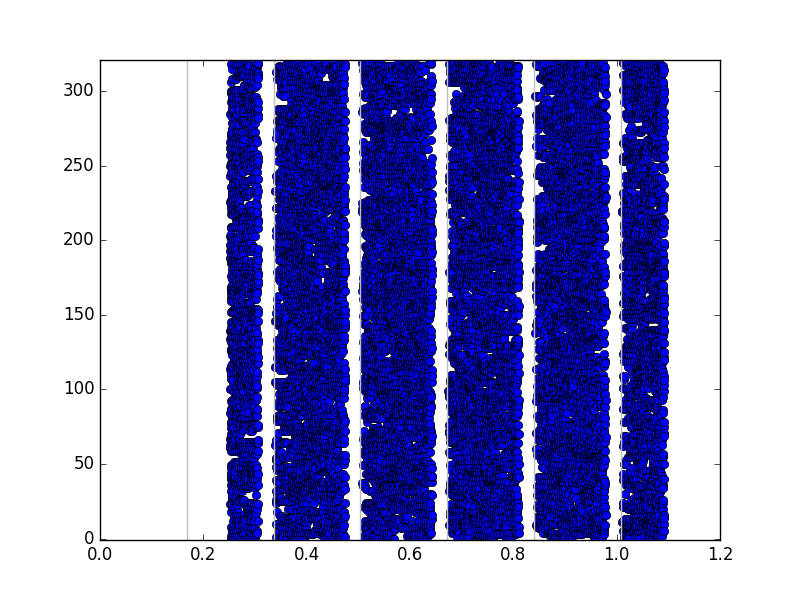
\includegraphics[width=.9\linewidth]{imgs/app/inhib_no.png}
  		\caption{Spikes without lateral inhibition.}
  		\label{fig:sub1}
	\end{subfigure}%
	
	\begin{subfigure}[t]{.55\textwidth}
  		\centering
  		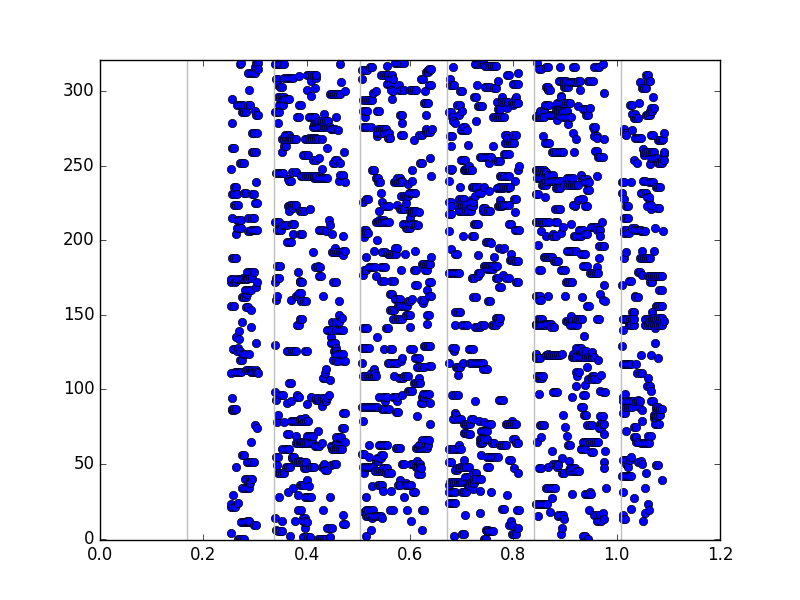
\includegraphics[width=.9\linewidth]{imgs/app/inhib_small.png}
  		\caption{Spikes with small lateral inhibition.}
  		\label{fig:sub2}
	\end{subfigure}
	
	\begin{subfigure}[t]{.55\textwidth}
  		\centering
  		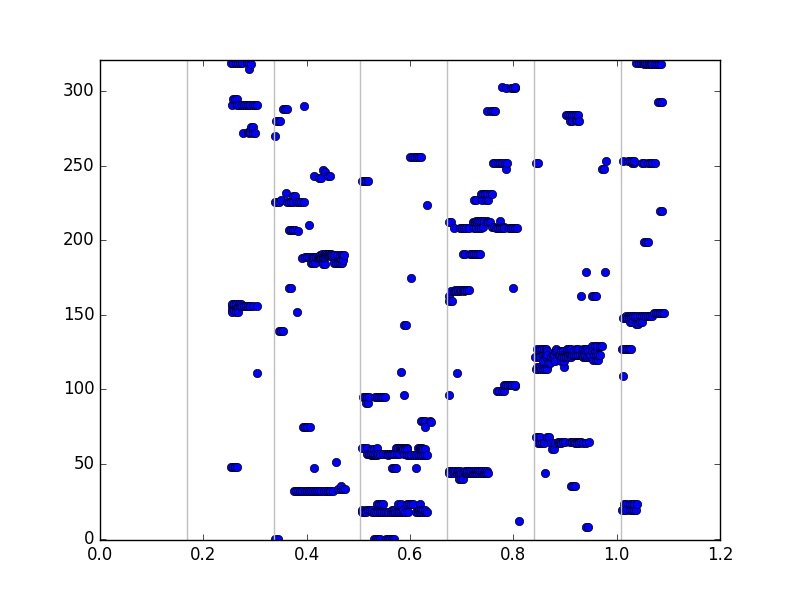
\includegraphics[width=.9\linewidth]{imgs/app/inhib_big.png}
  		\caption{Spikes with big lateral inhibition.}
  		\label{fig:sub2}
	\end{subfigure}
	\caption[Spikes in a hidden layer of a spiking RBM with different kinds of lateral inhibition.]{Spikes in a hidden layer of a spiking RBM with lateral inhibition. As the lateral inhibition increases, the activity becomes more sparse. In the case with big inhibitory weights, there are a few neurons dominating the activity allowing only a few different states of the network and thus poor mode switching in a training step. In a network with small inhibitory weights, there is sparse activity, but the the network visits many different states in a simulation step and shows sufficient mode mixing. }
	\label{fig:dbnmixing}
\end{figure}
   
\section{Spiking DBN Architectures}   
   
 \begin{figure}[h!]
	\centering
	\begin{subfigure}[t]{.49\textwidth}
  		\centering
  		
\includegraphics[width=.4\linewidth]{imgs/spike_dbn.png}
  		\label{fig:sub1}
  		\caption{DBN with distinct RBM layers.}
	\end{subfigure}%
	\begin{subfigure}[t]{.49\textwidth}
  		\centering
  		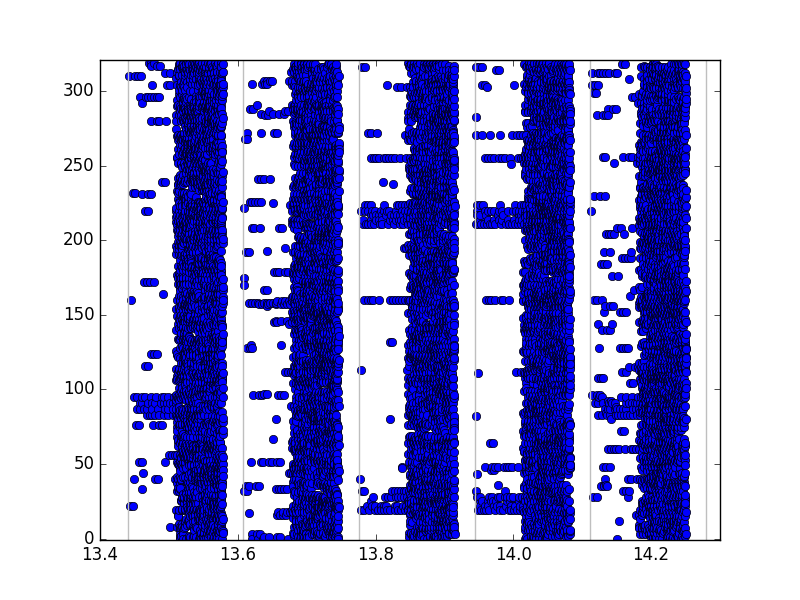
\includegraphics[width=.9\linewidth]{imgs/app/DBN_sp.png}
  		\label{fig:sub1}
	\end{subfigure}%
	
	
	\begin{subfigure}[t]{.49\textwidth}
  		\centering
  		
\includegraphics[width=.4\linewidth]{imgs/spike_dbm.png}
  		\label{fig:sub1}
  		\caption{DBN with distinct RBM layers, with bidirectional weights.}
	\end{subfigure}%
	\begin{subfigure}[t]{.49\textwidth}
  		\centering
  		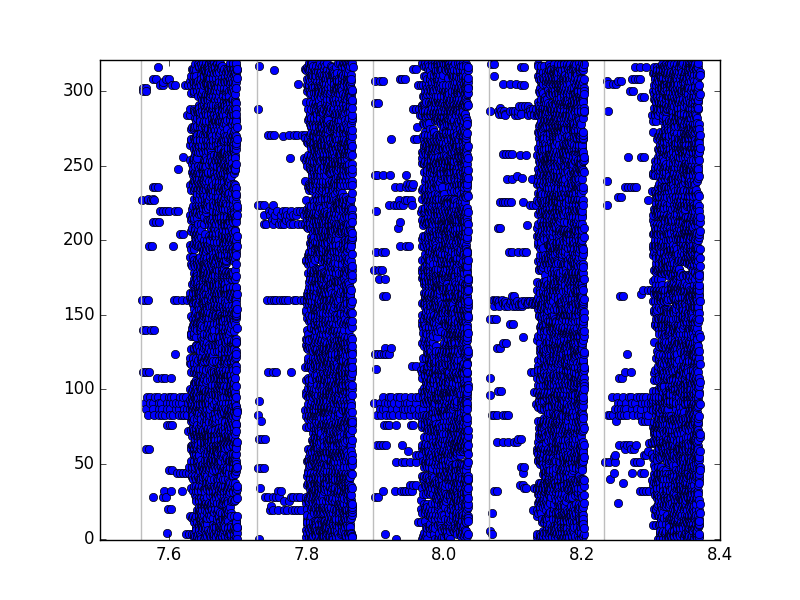
\includegraphics[width=.9\linewidth]{imgs/app/DBM_sp.png}
  		\label{fig:sub2}
	\end{subfigure}
	
	
	\begin{subfigure}[t]{.49\textwidth}
  		\centering
  		
\includegraphics[width=.50\linewidth]{imgs/app/dbn_np_arch.png}
  		\label{fig:sub1}
  		 \caption{DBN with RBM directly stacked to each other.}
	\end{subfigure}%
	\begin{subfigure}[t]{.49\textwidth}
  		\centering
  		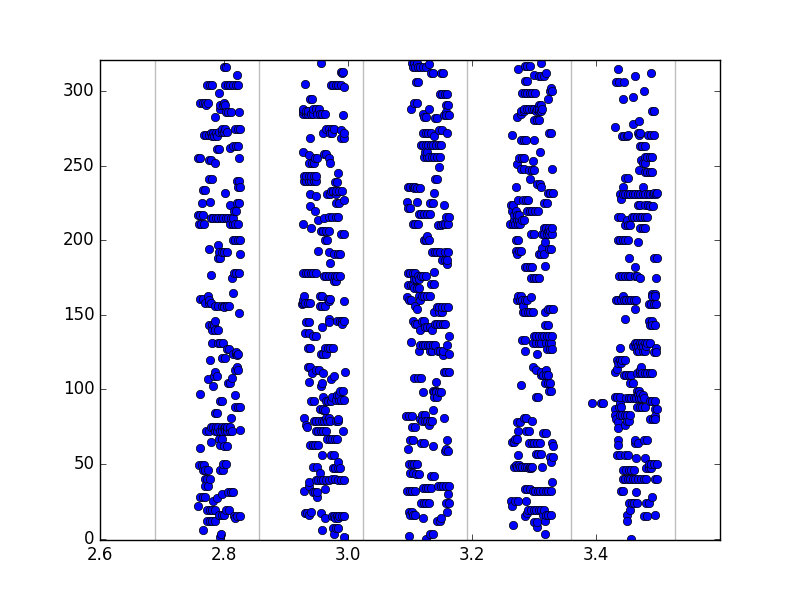
\includegraphics[width=.9\linewidth]{imgs/app/DBN_np_sp.png}
  		\label{fig:sub2}
	\end{subfigure}
	\caption[Activity in the visible layer of the top RBM in a DBNs with different architectures.]{Activity in the visible layer of the top RBM in a DBNs with different architectures. The first two architectures model separate RBM layers which are stacked by one-on-one forward connections from the hidden layer of the bottom RBM to the visible layer of the top RBM, while in the last architecture, the RBMs are directly stacked, i.e. the hidden layer of the bottom RBM is the visible layer of the top RBM. While in the top two architectures, there are hardly any differences and the input is modelled correctly, due to top down influences the output of the bottom RBM gets distorted by activity in the hidden layer of the top RBM.}
	\label{fig:spikingdbnarch}
\end{figure}

\section{Synchronous Weight Updates} \label{fig:ecdnestconv}

For this thesis two different approaches were implemented. 

The first approach, as presented in Chapter \ref{c:ecdconv} and \ref{c:ecdexp}, synchronizes the weights at a discrete time step after a training sample is presented and processed.
This poses some similarities to the normal contrastive divergence algorithm since, due to discrete nature of artificial neural networks, the weights are updated and synchronized after the positive and negative phase.  

The second approach keeps the weights synchronized by applying the same STDP update to all synapses which share the same weight at the same time. 
Namely, if one synapses is updated by a local STDP rule, the update is shared with all tied synapses.
For the non-convolutional case i.e. only the weights of forward and backward synapses between the same neurons are shared, this leads to discriminative results, as shown in Figure \ref{fig:nestwwout}.

\begin{figure}[h!]

	\begin{subfigure}[t]{.49\textwidth}
		\centering
		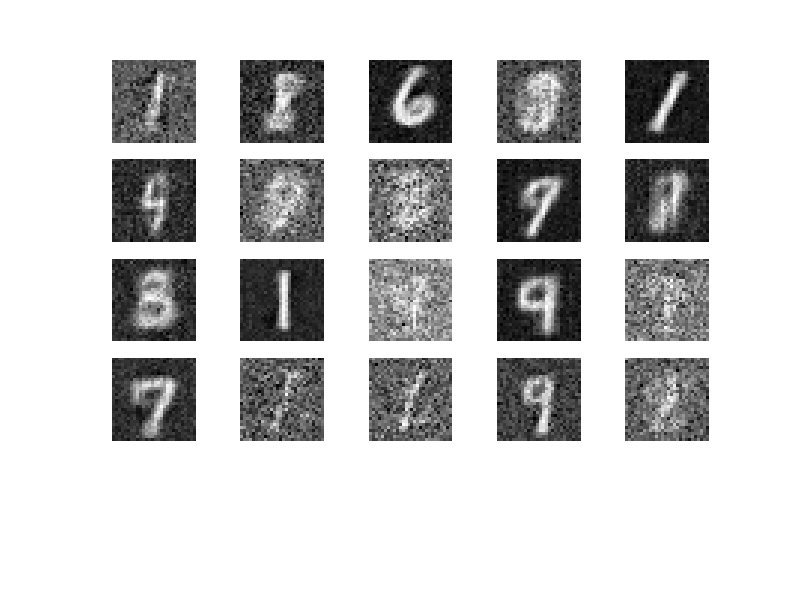
\includegraphics[width=.9\linewidth]{imgs/app/nest/ws.png}
		\caption{}
		\label{fig:sub12}
	\end{subfigure}
	\begin{subfigure}[t]{.49\textwidth}
  		\centering
  		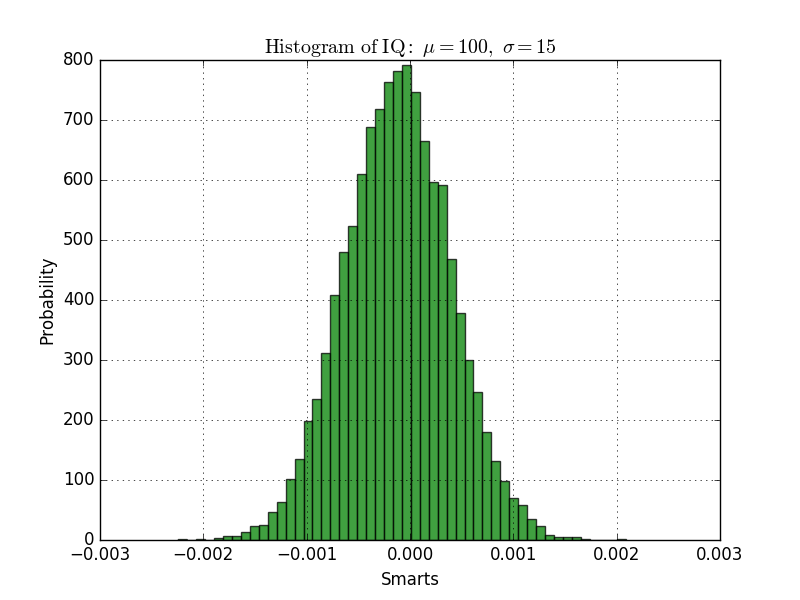
\includegraphics[width=.9\linewidth]{imgs/app/nest/w_hist_normal.png}
  		\caption{}
  		\label{fig:sub2}
	\end{subfigure}
	\caption[Weights with shared STDP weight updates and without any convolution.]{Weights with shared STDP weight updates and without any convolution. The weights are visualized in (a) as the filter matrices and in (b) as a histogram. }
	\label{fig:nestwwout}
\end{figure}	


In our case, the case with shared STDP updates with convolutions did not show any promising results. Although the learning rate was scaled accordingly, due to some self-facilitation and weight explosion, the weights become mostly negative as illustrated in Figure \ref{fig:ecdnestconv}.


 \begin{figure}[h!]
	\centering
	\begin{subfigure}[t]{.24\textwidth}
  		\centering
  		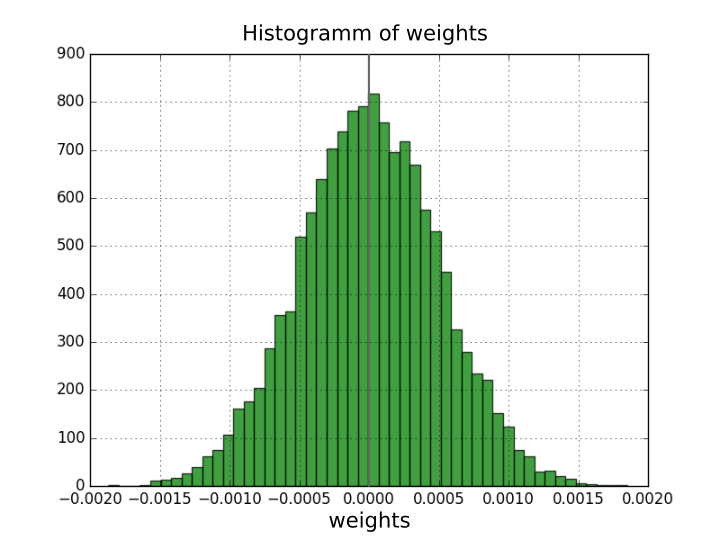
\includegraphics[width=.9\linewidth]{imgs/app/nest/w_hist_conv1.png}
  		\caption{}
  		\label{fig:sub1}
	\end{subfigure}%
	\begin{subfigure}[t]{.24\textwidth}
  		\centering
  		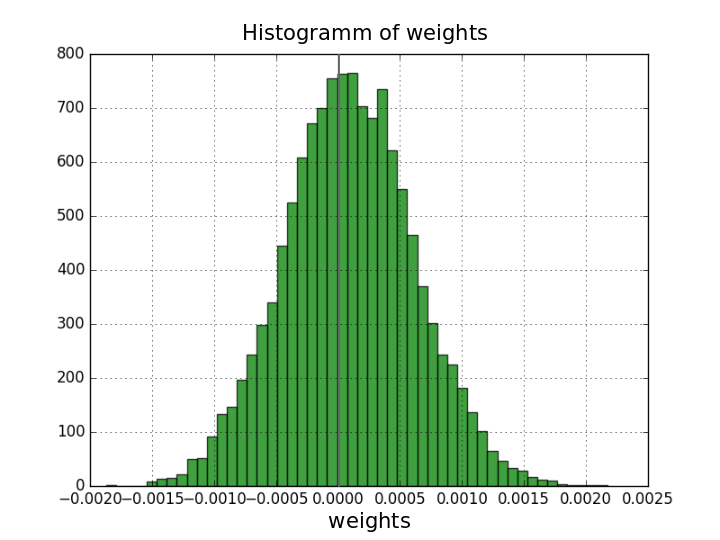
\includegraphics[width=.9\linewidth]{imgs/app/nest/w_hist_conv2.png}
  		\caption{}
  		\label{fig:sub2}
	\end{subfigure}
	\begin{subfigure}[t]{.24\textwidth}
  		\centering
  		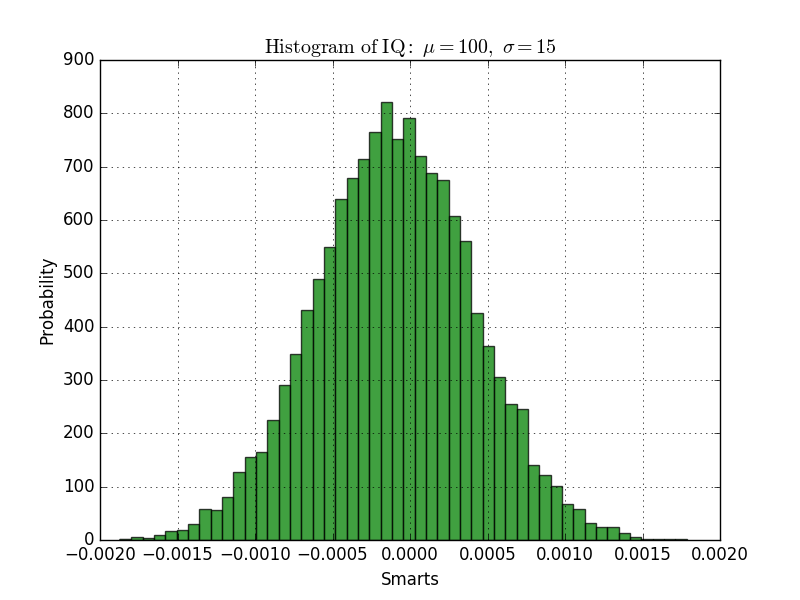
\includegraphics[width=.9\linewidth]{imgs/app/nest/w_hist_conv3.png}
  		\caption{}
  		\label{fig:sub2}
	\end{subfigure}
	\begin{subfigure}[t]{.24\textwidth}
  		\centering
  		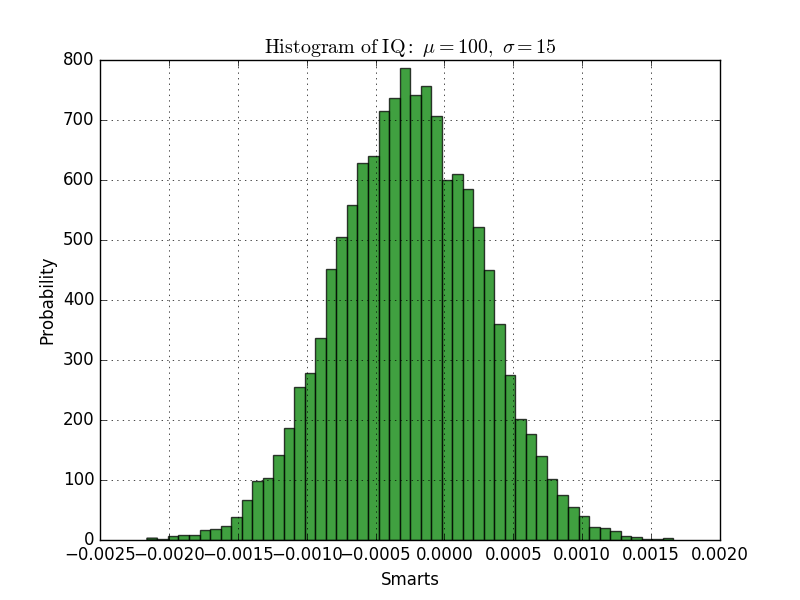
\includegraphics[width=.9\linewidth]{imgs/app/nest/w_hist_conv4.png}
  		\caption{}
  		\label{fig:sub2}
	\end{subfigure}
	\caption[Weights development for eCD with synchronous weight updates.]{Weights development for eCD with synchronous weight updates. The weight distribution in the beginning is shown in (a). After the positive phase (b) the weights increased a lot, which leads to a high decrement during the negative (c). During further training this trend continues until most weights are negative (d).}
	\label{fig:ecdnestconv}
\end{figure}

As a result, due to the mostly negative weights, this leads to a "dying-out" of the spike activity which is shown in Figure \ref{fig:ecdnestdieout} 

\begin{figure}[h!]
 	\centering
  	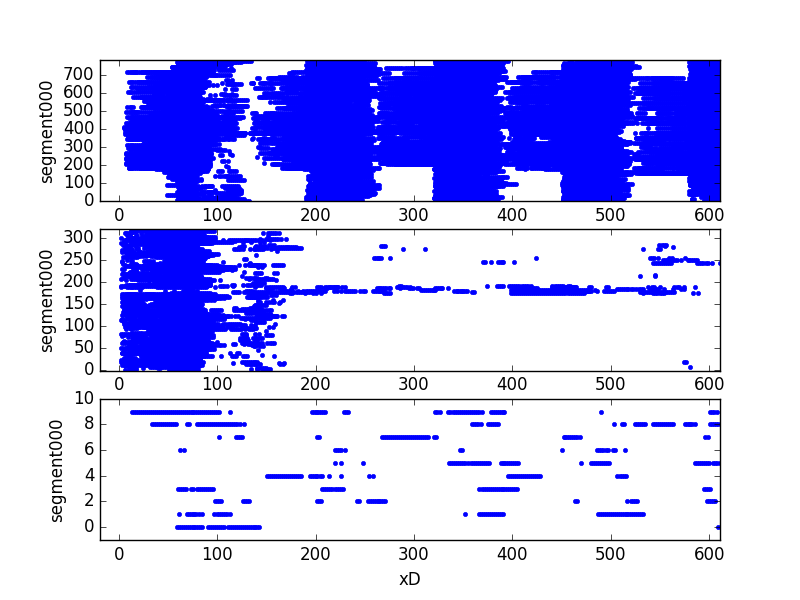
\includegraphics[width=.4\linewidth]{imgs/app/nest/spikes_conv.png}
  	\caption[Spikes activity during convolutional eCD with synchronous weight updates.]{Spikes activity during convolutional eCD with synchronous weight updates. After a few training samples are presented the spiking activity decreases, due to the decrement of the synaptic weights.}
  	\label{fig:ecdnestdieout}
\end{figure}

Thus, no learning happens and the weights become not very discriminative (compare Figure \ref{fig:ecdnestwnot}).


\begin{figure}[h!]
 	\centering
  	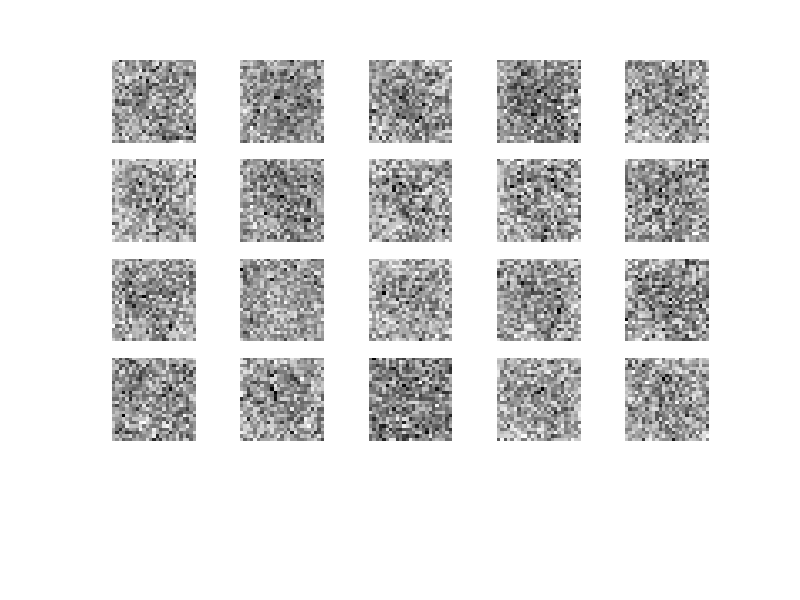
\includegraphics[width=.4\linewidth]{imgs/app/nest/w_not.png}
  	\caption{Learned weights for convolutional eCD with synchronous weight updates.}
  	\label{fig:ecdnestwnot}
\end{figure}

Increasing the learning rate to increase the weights leads to a few strong positive weights, while the majority of the weights still become negative, leading to no good results either (Fig. \ref{fig:ecdnestwnot}).


\begin{figure}[h!]
 	\centering
  	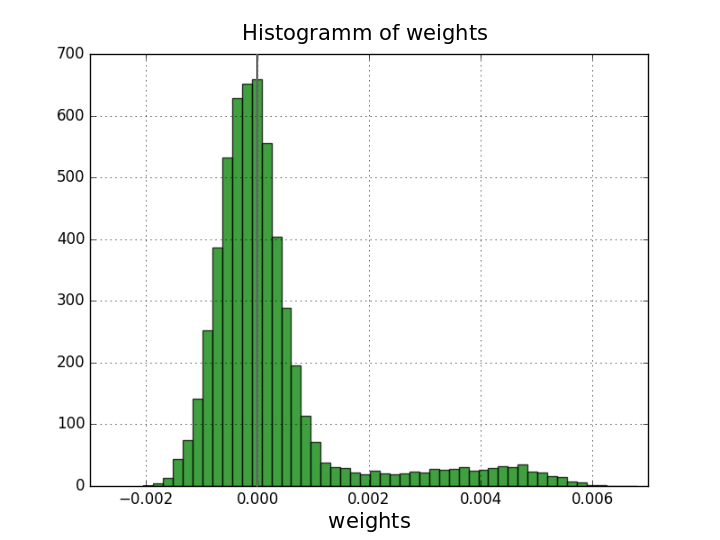
\includegraphics[width=.4\linewidth]{imgs/app/nest/w_hist_conv_lr.png}
  	\caption[Weight histogram for convolutional eCD with synchronous weight updates and an increased learning rate during the positive phase.]{Weight histogram for convolutional eCD with synchronous weight updates and an increased learning rate during the positive phase. This leads to a division of the weights into a few very positive weights and many negative weights. }
  	\label{fig:ecdnestwnot}
\end{figure}

Further research on this topic could indicate whether a fine-tuned learning rate or a dynamic learning rate decay or adaptation could be a sound remedy to this problem. 

%
% \begin{figure}[h!]
%	\centering
%	\begin{subfigure}[t]{.24\textwidth}
%  		\centering
%  		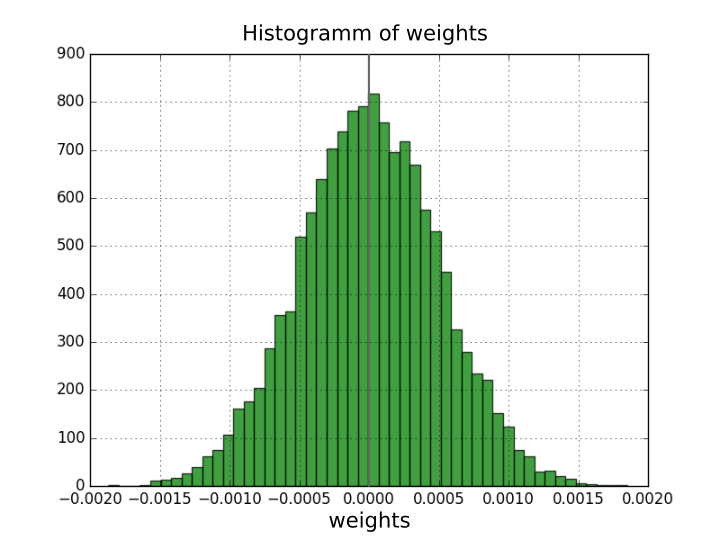
\includegraphics[width=.9\linewidth]{imgs/app/nest/w_hist_conv1.png}
%  		\caption{Weights at the beginning.}
%  		\label{fig:sub1}
%	\end{subfigure}%
%	\begin{subfigure}[t]{.24\textwidth}
%  		\centering
%  		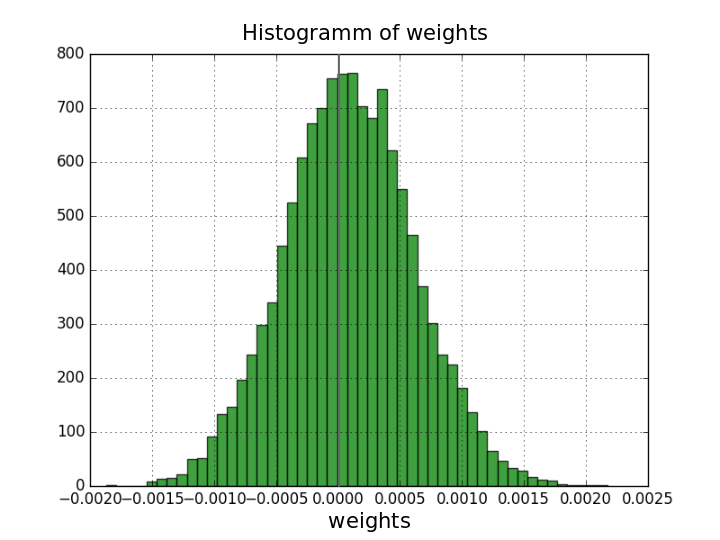
\includegraphics[width=.9\linewidth]{imgs/app/nest/w_hist_conv2.png}
%  		\caption{Weights after first positive phase.}
%  		\label{fig:sub2}
%	\end{subfigure}
%	\begin{subfigure}[t]{.24\textwidth}
%  		\centering
%  		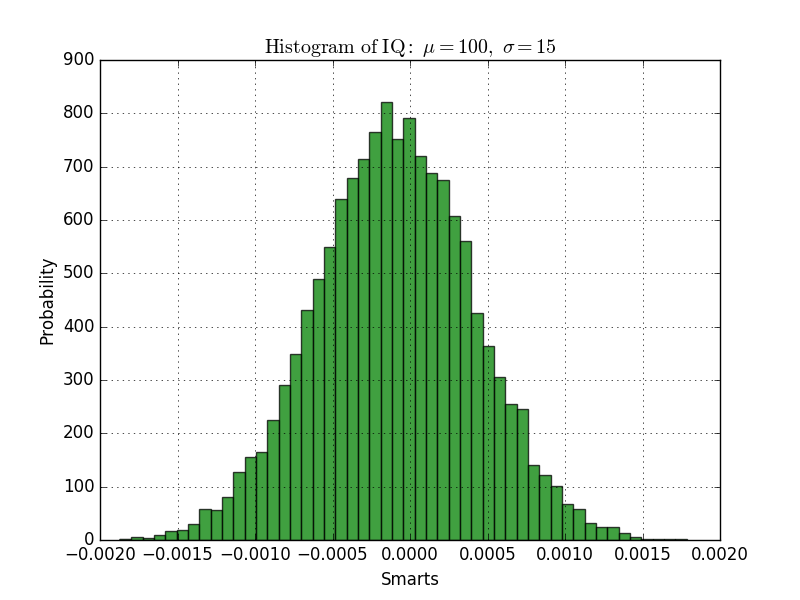
\includegraphics[width=.9\linewidth]{imgs/app/nest/w_hist_conv3.png}
%  		\caption{Weights after first negative phase.}
%  		\label{fig:sub2}
%	\end{subfigure}
%	\begin{subfigure}[t]{.24\textwidth}
%  		\centering
%  		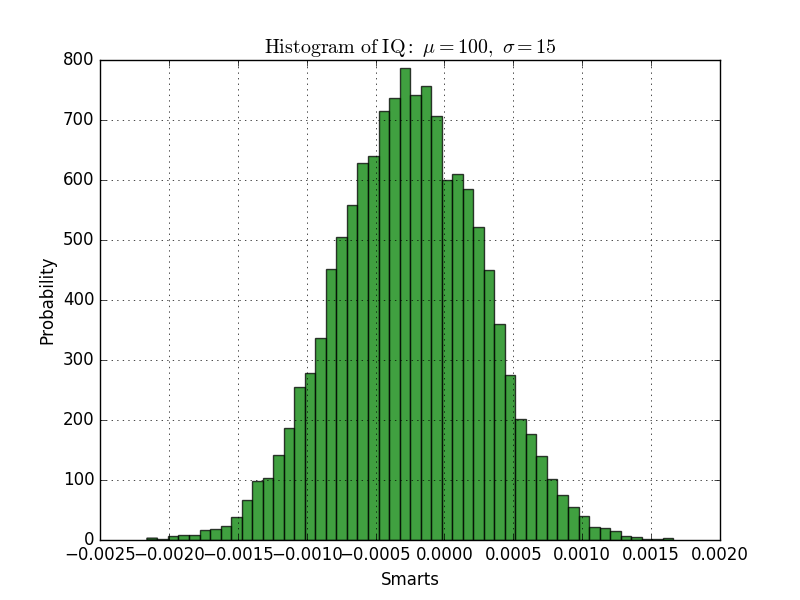
\includegraphics[width=.9\linewidth]{imgs/app/nest/w_hist_conv4.png}
%  		\caption{Weights after a few training steps.}
%  		\label{fig:sub2}
%	\end{subfigure}
%	
%
%	\begin{subfigure}[t]{.24\textwidth}
%  		\centering
%  		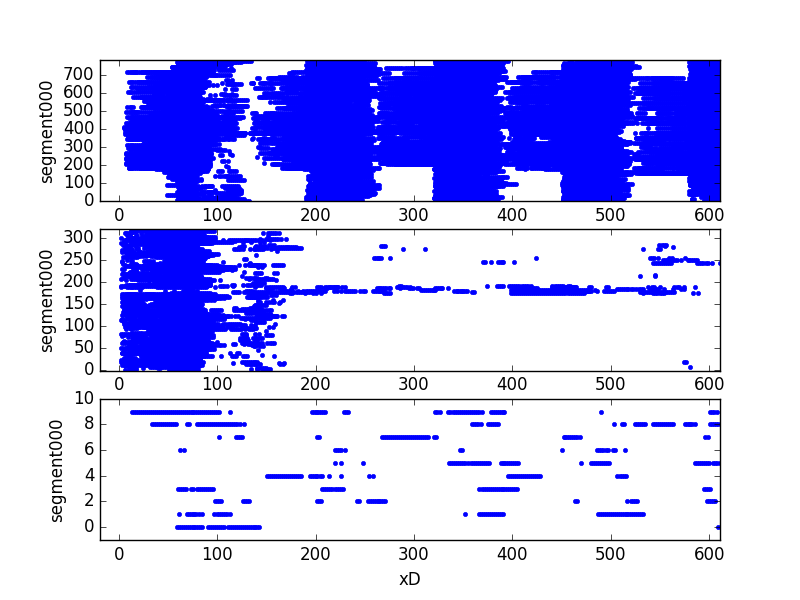
\includegraphics[width=.9\linewidth]{imgs/app/nest/spikes_conv.png}
%  		\caption{Spikes activity development.}
%  		\label{fig:sub2}
%	\end{subfigure}
%	
%	
%	\begin{subfigure}[t]{.24\textwidth}
%  		\centering
%  		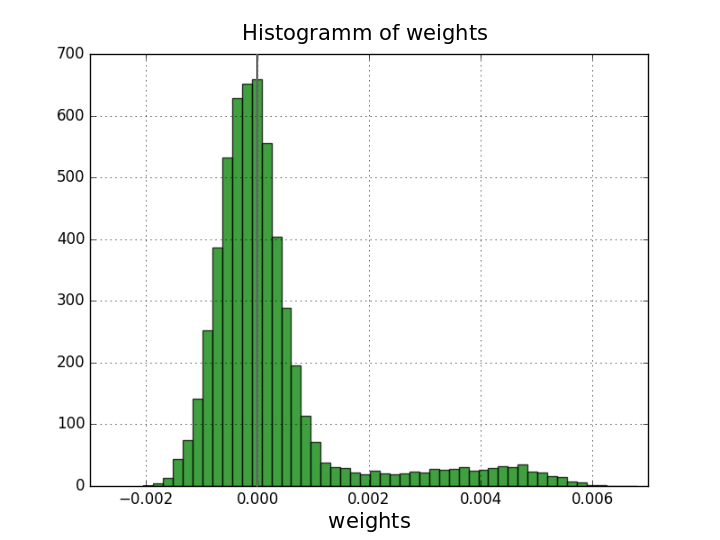
\includegraphics[width=.9\linewidth]{imgs/app/nest/w_hist_conv_lr.png}
%  		\caption{Weights after training with different positive and negative learning rates.}
%  		\label{fig:sub2}
%	\end{subfigure}
%	
%	\begin{subfigure}[t]{.24\textwidth}
%  		\centering
%  		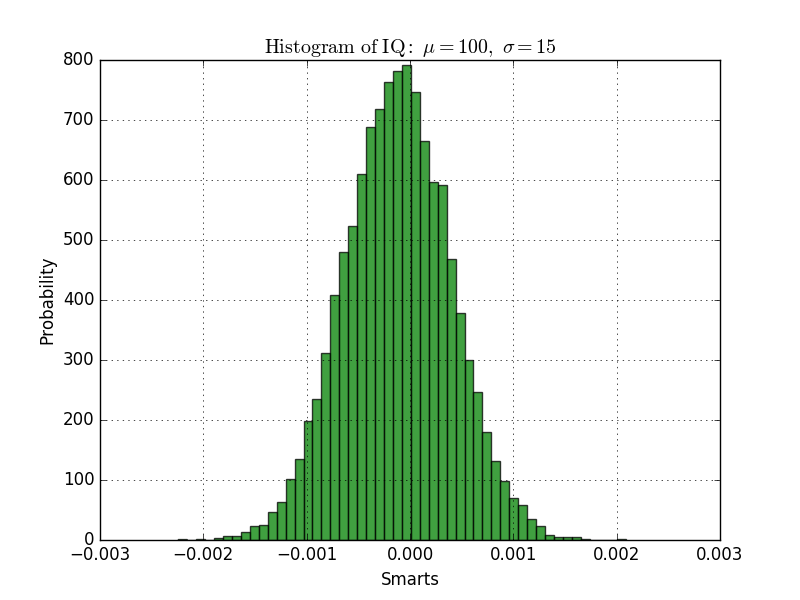
\includegraphics[width=.9\linewidth]{imgs/app/nest/w_hist_normal.png}
%  		\caption{Weights without any synchronization.}
%  		\label{fig:sub2}
%	\end{subfigure}	
%	
%	\caption{Weights development for eCD with synchronous weight updates. The first column shows the development. After the positive the weights increased a lot, which leads to a high decrement during the negative which leads to a "dying out" of the spikes, which is visualized in the second column. Using an increased positive phase with a higher learning rate, does not solve the problem and leads to a division of the weights into a few very positive weights and many negative weights. In contrast to this a "normal" weight distribution without any weight synchronization in presented in the last column. }
%	\label{fig:ecdnestconv}
%\end{figure}



\listoftodos
\listoffigures
\listoftables
\bibliography{content/bibliography}

\printindex


\end{document}
